% LaTeX source for ``Think DSP: Digital Signal Processing for Programmers''
% Copyright 2013  Allen B. Downey.

% License: Creative Commons Attribution-NonCommercial 3.0 Unported License.
% http://creativecommons.org/licenses/by-nc/3.0/
%

\documentclass[12pt]{book}
\usepackage[width=5.5in,height=8.5in,
  hmarginratio=3:2,vmarginratio=1:1]{geometry}

% for some of these packages, you might have to install
% texlive-latex-extra (in Ubuntu)

\usepackage[T1]{fontenc}
\usepackage{textcomp}
\usepackage{mathpazo}
\usepackage{url}
\usepackage{graphicx}
\usepackage{subfig}
\usepackage{amsmath}
\usepackage{amsthm}
\usepackage{makeidx}
\usepackage{setspace}
\usepackage{hevea}                           
\usepackage{upquote}
\usepackage{fancyhdr}
\usepackage[bookmarks]{hyperref}

\title{Think DSP}
\author{Allen B. Downey}

\newcommand{\thetitle}{Think DSP: Digital Signal Processing in Python}
\newcommand{\theversion}{0.4}

% these styles get translated in CSS for the HTML version
\newstyle{a:link}{color:black;}
\newstyle{p+p}{margin-top:1em;margin-bottom:1em}
\newstyle{img}{border:0px}

% change the arrows in the HTML version
\setlinkstext
  {\imgsrc[ALT="Previous"]{back.png}}
  {\imgsrc[ALT="Up"]{up.png}}
  {\imgsrc[ALT="Next"]{next.png}} 

\makeindex

\newif\ifplastex
\plastexfalse

\begin{document}

\frontmatter

\ifplastex

\else
\fi

\ifplastex
    \usepackage{localdef}
    \maketitle

\else

\newtheoremstyle{exercise}% name of the style to be used
  {\topsep}% measure of space to leave above the theorem. E.g.: 3pt
  {\topsep}% measure of space to leave below the theorem. E.g.: 3pt
  {}% name of font to use in the body of the theorem
  {0pt}% measure of space to indent
  {\bfseries}% name of head font
  {}% punctuation between head and body
  { }% space after theorem head; " " = normal interword space
  {}% Manually specify head

\theoremstyle{exercise}
\newtheorem{exercise}{Exercise}[chapter]

\input{latexonly}

\begin{latexonly}

\renewcommand{\blankpage}{\thispagestyle{empty} \quad \newpage}

% TITLE PAGES FOR LATEX VERSION

%-half title--------------------------------------------------
\thispagestyle{empty}

\begin{flushright}
\vspace*{2.0in}

\begin{spacing}{3}
{\huge Think DSP}\\
{\Large Digital Signal Processing in Python}
\end{spacing}

\vspace{0.25in}

Version \theversion

\vfill

\end{flushright}

%--verso------------------------------------------------------

\blankpage
\blankpage

%--title page--------------------------------------------------
\pagebreak
\thispagestyle{empty}

\begin{flushright}
\vspace*{2.0in}

\begin{spacing}{3}
{\huge Think DSP}\\
{\Large Digital Signal Processing in Python}
\end{spacing}

\vspace{0.25in}

Version \theversion

\vspace{1in}


{\Large
Allen B. Downey\\
}


\vspace{0.5in}

{\Large Green Tea Press}

{\small Needham, Massachusetts}

\vfill

\end{flushright}


%--copyright--------------------------------------------------
\pagebreak
\thispagestyle{empty}

Copyright \copyright ~2013 Allen B. Downey.


\vspace{0.2in}

\begin{flushleft}
Green Tea Press       \\
9 Washburn Ave \\
Needham MA 02492
\end{flushleft}

Permission is granted to copy, distribute, and/or modify this document
under the terms of the Creative Commons Attribution-NonCommercial 3.0 Unported
License, which is available at \url{http://creativecommons.org/licenses/by-nc/3.0/}.

\vspace{0.2in}

\end{latexonly}


% HTMLONLY

\begin{htmlonly}

% TITLE PAGE FOR HTML VERSION

{\Large \thetitle}

{\large Allen B. Downey}

Version \theversion

\vspace{0.25in}

Copyright 2012 Allen B. Downey

\vspace{0.25in}

Permission is granted to copy, distribute, and/or modify this document
under the terms of the Creative Commons Attribution-NonCommercial 3.0
Unported License, which is available at
\url{http://creativecommons.org/licenses/by-nc/3.0/}.

\setcounter{chapter}{-1}

\end{htmlonly}

\fi
% END OF THE PART WE SKIP FOR PLASTEX

\chapter{Preface}
\label{preface}

The premise of this book (and the other books in the {\it Think X}
series) is that if you know how to program, you can use that skill to
learn other things.  I am writing this book because I think the
conventional approach to digital signal processing is backward: most
books (and the classes that use them) present the material bottom-up,
starting with mathematical abstractions like phasors.

With a programming-based approach, I can go top-down, which means I
can present the most important ideas right away.  By the end of the
first chapter, you can break down a sound into its harmonics, modify
the harmonics, and generate new sounds.

This is a work in progress, so comments are welcome.


Allen B. Downey \\*

Needham MA \\*

Allen B. Downey is a Professor of Computer Science at 
the Franklin W. Olin College of Engineering.



\section*{Contributor List}

If you have a suggestion or correction, please send email to 
{\tt downey@allendowney.com}.  If I make a change based on your
feedback, I will add you to the contributor list
(unless you ask to be omitted).
\index{contributors}

If you include at least part of the sentence the
error appears in, that makes it easy for me to search.  Page and
section numbers are fine, too, but not as easy to work with.
Thanks!

\small

\begin{itemize}

\item 

% ENDCONTRIB

\end{itemize}

\normalsize

\clearemptydoublepage

% TABLE OF CONTENTS
\begin{latexonly}

\tableofcontents

\clearemptydoublepage

\end{latexonly}

% START THE BOOK
\mainmatter


\chapter{Sounds and signals}
\label{sounds}

A {\bf signal} is a representation of a quantity that varies in time,
or space, or both.  That definition is pretty abstract, so let's start
with a concrete example, sound.  Sound is variation in air pressure.
A sound signal represents variations in air pressure over time.

A microphone is a device that measures these variations and generates
an electronic signal that represents sound.  A speaker is a device
that takes an electrical signal and produces sound.
Microphones and speakers are called {\bf transducers} because they
transduce, or convert, signals from one form to another.

This book is about signal processing, which includes processes for
synthesizing, transforming, and analyzing signals.  It focuses on
sound signals, but the same methods apply to other signals, like
electronic signals and mechanical vibration.

They also apply to signals that vary in space rather than time, like
elevation along a hiking trail.  And they apply to signals in more
than one dimension, like an image, which you can think of as a signal
that varies in two-dimensional space.  Or a movie, which is
a signal that varies in two-dimensional space {\it and} time.

But we start with simple one-dimensional sound.


\section{Periodic signals}

\begin{figure}
% violin.py
\centerline{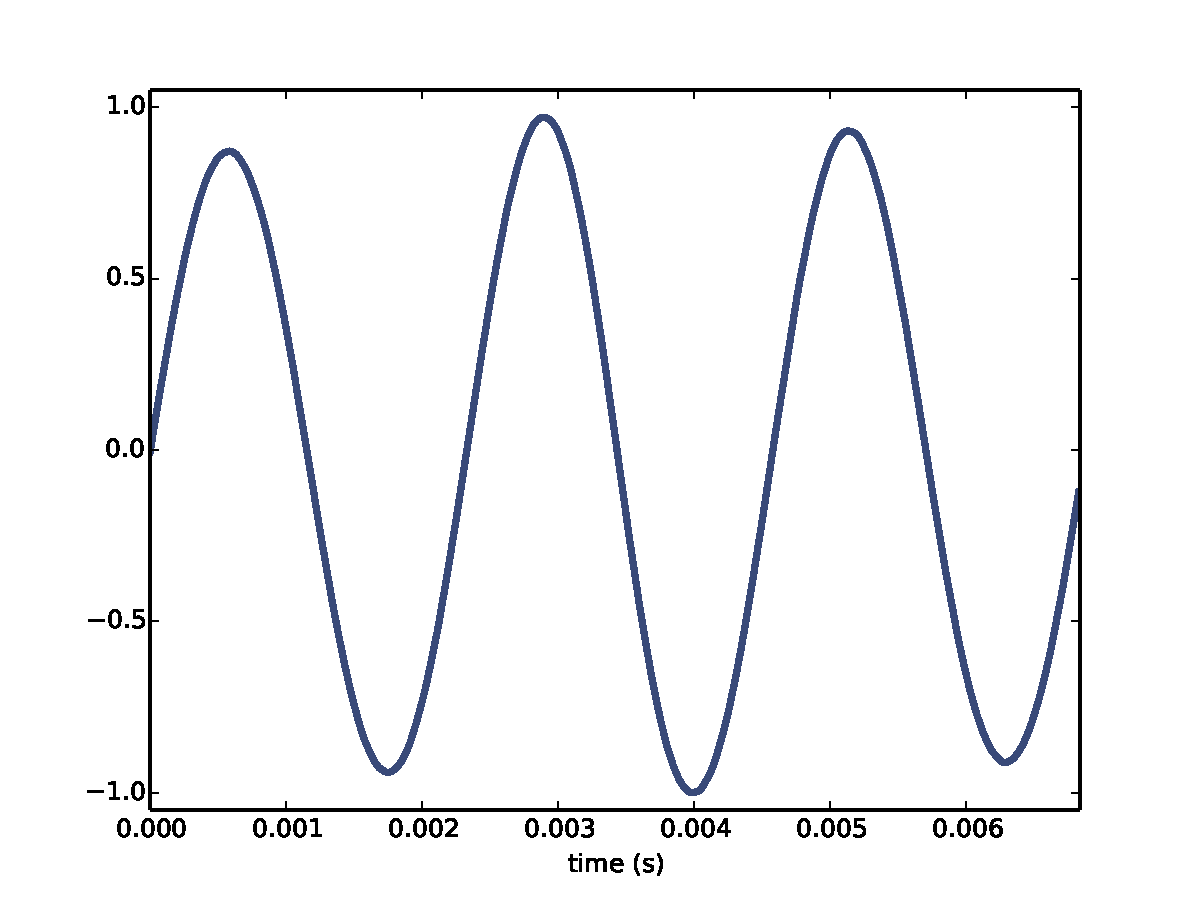
\includegraphics[height=2.5in]{figs/tuning1.pdf}}
\caption{Segment from a recording of a tuning fork.}
\label{fig.tuning1}
\end{figure}

We'll also start with {\bf periodic signals}, which are signals that
repeat themselves after some period of time.  For example, if you
strike a tuning fork, it vibrates and generates sound.  If you record
that sound and plot the transduced signal, it looks like
Figure~\ref{fig.tuning1}.\footnote{I got this recording from
  \url{http://www.freesound.org/people/zippi1/sounds/18871/}.}

This signal is a sinusoid, which means it has the same shape as
the trigonometric sine function. 

You can see that this signal is periodic.  I chose the duration
to show three full periods, also known as {\bf cycles}.
The duration of each cycle is
about 2.3 ms.

The {\bf frequency} of a signal is the number of cycles
per second, which is the inverse of the period.
The units of frequency are cycles per second, or {\bf Hertz},
abbreviated ``Hz''.

The frequency of this signal is about 439 Hz, slightly lower than 440
Hz, which is the standard tuning pitch for orchestral music.  The
musical name of this note is A, or more specifically, A4.  If you are
not familiar with ``scientific pitch notation'', the suffix indicates
which octave the note is in.  A4 is the A above middle C.  A5 is one
octave higher.  See
\url{http://en.wikipedia.org/wiki/Scientific_pitch_notation}.

\begin{figure}
% violin.py
\centerline{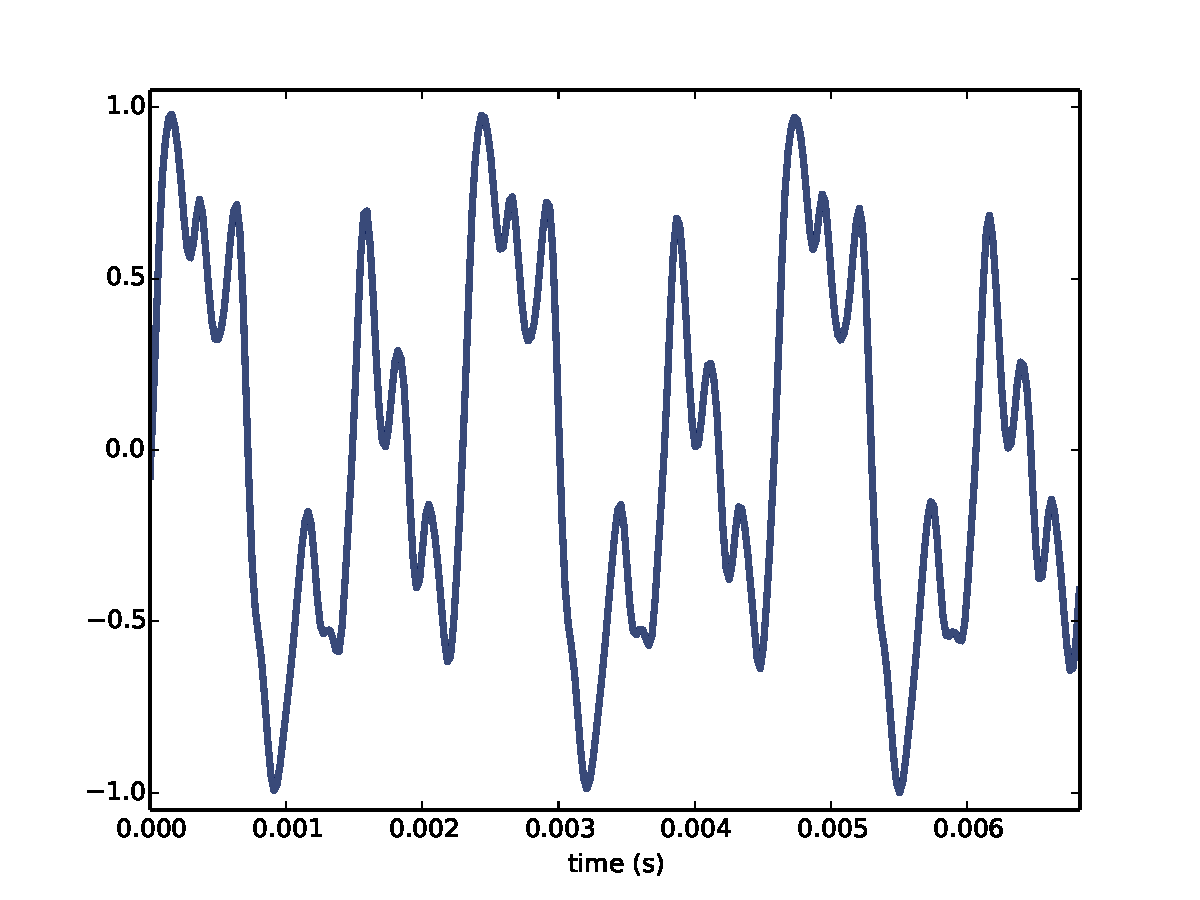
\includegraphics[height=2.5in]{figs/violin1.pdf}}
\caption{Segment from a recording of a violin.}
\label{fig.violin1}
\end{figure}

A tuning fork generates a sinusoid because the vibration of the tines
is a form of simple harmonic motion.  Most musical instruments
produce periodic signals, but the shape of these signals is not
sinusoidal.  For example, Figure~\ref{fig.violin1} shows a segment
from a recording of a violin playing
Boccherini's String Quintet No. 5 in E, 3rd
movement.\footnote{The recording is from
  \url{http://www.freesound.org/people/jcveliz/sounds/92002/}.
I identified the piece using \url{http://www.musipedia.org}.}

% Parson's code: DUUDDUURDR

Again we can see that the signal is periodic, but the shape of the
signal is much more complex.  The shape of a periodic signal is called
the {\bf waveform}.  Most musical instruments produce waveforms more
complex than a sinusoid.  The shape of the waveform determines the
musical {\bf timbre}, which is our perception of the tone quality of the
sound.  People usually perceive complex waveforms as rich, warm and
more interesting than sinusoids.


\section{Spectral decomposition}

\begin{figure}
% violin.py
\centerline{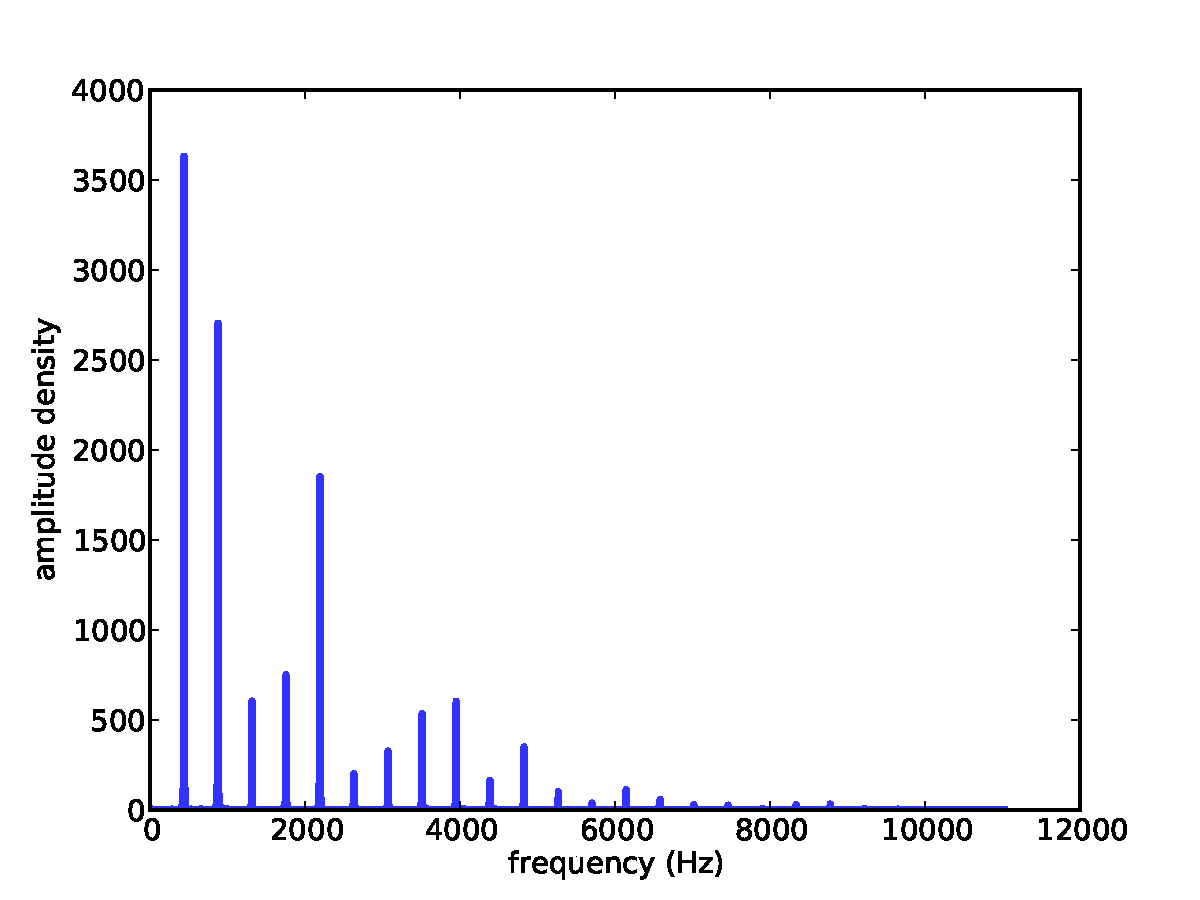
\includegraphics[height=2.5in]{figs/violin2.pdf}}
\caption{Spectrum of a segment from the violin recording.}
\label{fig.violin2}
\end{figure}

The most important idea in this book is {\bf spectral decomposition},
which is the idea that a complex signal can be expressed as the sum of
simpler signals with different frequencies.

And the most important algorithm in this book is the {\bf discrete
  Fourier transform}, or {\bf DFT}, which takes a signal (a quantity
varying in time) and produces its {\bf spectrum}, which is the set of
sinusoids that add up to produce the signal.

For example, Figure~\ref{fig.violin2} shows the spectrum of the violin
recording in Figure~\ref{fig.violin1}.  The x-axis is the range of
frequencies that make up the signal.  The y-axis shows the strength of
each frequency component.

The lowest frequency component is called the {\bf fundamental
  frequency}.  The fundamental frequency of this signal is near 440 Hz
(actually a little lower, or ``flat'').

In this signal the fundamental frequency has the largest amplitude,
so it is also the {\bf dominant frequency}.

Normally the perceived pitch of a sound is determined by the
fundamental frequency, even if it is not dominant. 

The other spikes in the spectrum are at frequencies 880, 1320, 1760, and
2200, which are integer multiples of the fundamental.
These components are called {\bf harmonics} because they are
musically harmonious with the fundamental:

\begin{itemize}

\item 880 is the frequency of
A5, one octave higher than the fundamental.  

\item 1320 is approximately E6, which is a major fifth above A5.

\item 1760 is A6, two octaves above the fundamental. 

\item 2200 is approximately C$\sharp$7, which is a major third
above A6.

\end{itemize}

In other words, these harmonics make up the notes of an A major
chord, although not all in the same octave.  Some of them are only
approximate because the notes that make up Western music have been
adjusted for {\bf equal temperament} (see
 \url{http://en.wikipedia.org/wiki/Equal_temperament}).

Given the harmonics and their amplitudes, you can reconstruct the
signal (at least approximately) by adding up sinusoids.  Or, to
reconstruct the signal exactly, you can use the inverse DFT.  
Next we'll see how.


\section{Signals}

I wrote a Python module called {\tt thinkdsp} that contains
classes and function for working with signals and spectrums.
\footnote{In Latin the plural of ``spectrum'' is ``spectra'', but I
prefer to use standard English plurals.}  You can download
it from \url{http://think-dsp.com/thinkdsp.py}.

To represent signals, {\tt thinkdsp} provides a class named
{\tt Signal}, which is the parent class for several signal types,
including {\tt Sinusoid}, which represents both sine and cosine
signals.

{\tt thinkdsp} provides functions to create sine and cosine signals:

\begin{verbatim}
    cos_sig = thinkdsp.CosSignal(freq=440, amp=1.0, offset=0)
    sin_sig = thinkdsp.SinSignal(freq=880, amp=0.5, offset=0)
\end{verbatim}

{\tt freq} is frequency in Hz.  {\tt amp} is amplitude in arbitrary
units.  {\tt offset} is a {\tt phase offset} in radians.

The phase offset determines where in the period the signal starts
(that is, when {\tt t=0}).  For example, a cosine signal with {\tt
  offset=0} starts at $\cos 0$, which is 1.  With {\tt offset=pi/2} it
starts at $\cos \pi/2$, which is 0.
A sine signal with
{\tt offset=0} also starts at 0.  In fact,
a cosine signal with {\tt offset=pi/2} is identical to a sine
signal with {\tt offset=0}.

Signals have an \verb"__add__" method, so you can use the {\tt +}
operator to add them:

\begin{verbatim}
    mix = sin_sig + cos_sig
\end{verbatim}

The result is a {\tt SumSignal}, which represents the sum of two
or more signals.

A Signal is basically a Python representation of a mathematical
function.  Most signals are defined for all values of {\tt t},
from negative infinity to infinity.

But you can't do much with a
Signal until you evaluate it.
In this context, ``evaluate'' means taking a sequence of {\tt ts}
and computing the corresponding values of the signal, which I
call {\tt ys}.  I encapsulate {\tt ts} and {\tt ys} in an
object called a Wave.

A Wave represents a signal evaluated at a sequence of points in
time.  Each point in time is called a {\bf frame} (a term borrowed
from movies and video).  The measurement itself is called a
{\bf sample}, although ``frame'' and ``sample'' are sometimes
used interchangeably.

{\tt Signal} provides \verb"make_wave", which returns a new
Wave object:

\begin{verbatim}
    wave = mix.make_wave(duration=0.5, start=0, framerate=11025)
\end{verbatim}

{\tt duration} is the length of the Wave in seconds.  {\tt start} is
the start time, also in seconds.  {\tt framerate} is the (integer)
number of frames per second, which is also the number of samples
per second.

11,025 frames per second is one of several framerates commonly used in
audio file formats, including Waveform Audio File (WAV) and mp3. 

This example evaluates the signal from {\tt t=0} to {\tt t=0.5} at
5,513 equally-spaced frames (because 5,513 is half of 11,025).
The time between frames, or {\bf timestep}, is {\tt 1/11025} seconds, or
91 $\mu$s.

{\tt Wave} provides a {\tt plot} method that uses {\tt pyplot}.
You can plot the wave like this:

\begin{verbatim}
    wave.plot()
    pyplot.show()
\end{verbatim}

{\tt pyplot} is part of {\tt matplotlib}; it is included in many
Python distributions, or you might have to install it.

\begin{figure}
% example1.py
\centerline{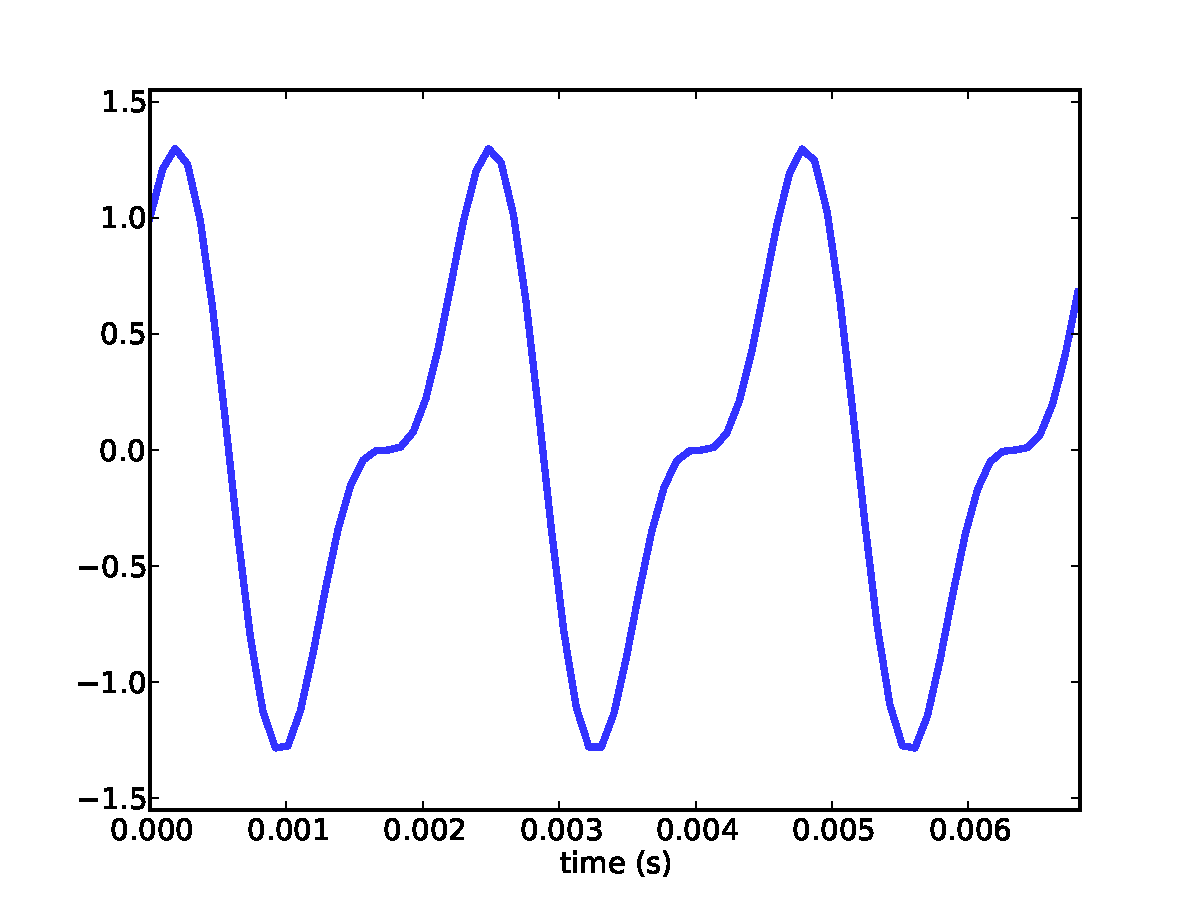
\includegraphics[height=2.5in]{figs/example1.pdf}}
\caption{Segment from a mixture of two sinusoid signals.}
\label{fig.example1}
\end{figure}

At {\tt freq=440} there are 220 periods in 0.5 seconds, so this plot
would look like a solid block of color.  To zoom in on a small number
of periods, we can use {\tt segment}, which copies a segment of a Wave
and returns a new wave:

\begin{verbatim}
    period = mix.period
    segment = wave.segment(start=0, duration=period*3)
\end{verbatim}

{\tt period} is a property of a Signal; it returns the period in second.

{\tt start} and {\tt duration} are in seconds.  This example copies
the first three periods from {\tt mix}.  If we plot {\tt segment}, it
looks like Figure~\ref{fig.example1}.  This signal contains two
frequency components, so it is more complex than the signal from the
tuning fork, but less complex than the violin.


\section{Reading and writing Waves}

{\tt thinkdsp} provides \verb"read_wave", which reads a WAV
file and returns a Wave:

\begin{verbatim}
    violin_wave = thinkdsp.read_wave('violin1.wav')
\end{verbatim}

And {\tt Wave} provides {\tt write}, which writes a WAV file:

\begin{verbatim}
    wave.write(filename='example1.wav')
\end{verbatim}

You can listen to the Wave with any media player that plays WAV
files.  On UNIX systems, I use {\tt aplay}, which is simple, robust,
and included in many Linux distributions.  For Windows you might like
MicroWav, available from
\url{http://bellsouthpwp2.net/b/o/bobad/microwav.htm}.

{\tt thinkdsp} also provides \verb"play_wave", which runs
the media player as a subprocess:

\begin{verbatim}
    thinkdsp.play_wave(filename='example1.wav', player='aplay')
\end{verbatim}

It uses {\tt aplay} by default, but you can provide another player.


\section{Spectrums}

{\tt Wave} provides \verb"make_spectrum", which returns a
{\tt Spectrum}:

\begin{verbatim}
    spectrum = wave.make_spectrum()
\end{verbatim}

And {\tt Spectrum} provides {\tt plot}:

\begin{verbatim}
    spectrum.plot()
    thinkplot.show()
\end{verbatim}

{\tt thinkplot} is a module I wrote to provide wrappers around some of
the functions in {\tt pyplot}.  You can download it from
\url{http://think-dsp.com/thinkplot.py}.  It is also included in the
Git repository for this book (see Section~\ref{code}).

{\tt Spectrum} provides three methods that modify the spectrum:

\begin{itemize}

\item \verb"low_pass" applies a low-pass filter, which means that
  components above a given cutoff frequency are attenuated (that is,
  reduced in magnitude) by a factor.

\item \verb"high_pass" applies a high-pass filter, which means that
  it attenuates components below the cutoff.

\item \verb"band_stop" attenuates components in a the band of
frequencies between two cutoffs.

\end{itemize}

This example attenuates all frequencies above 600 by 99\%:

\begin{verbatim}
   spectrum.low_pass(cutoff=600, factor=0.01)
\end{verbatim}

Finally, you can convert a Spectrum back to a Wave:

\begin{verbatim}
    wave = spectrum.make_wave()
\end{verbatim}

At this point you know how to use many of the classes and functions in
{\tt thinkdsp}, and you are ready to do the exercises at the end of
the chapter.  In Chapter~\ref{harmonics} I explain more
about how these classes are implemented.



\section{Exercises}

\begin{exercise}
Read the thinkdsp documentation.
\end{exercise}

\begin{exercise}
Fork and clone the repo.
\end{exercise}

\begin{exercise}
The example code in this chapter is in {\tt example1.py}.  If you
run it, it should ...

Gradually increase the cutoff and listen...
\end{exercise}

\begin{exercise}
Run violin.py and listen.
\end{exercise}

\begin{exercise}
Create exercise1.py and copy example1.py

Record a WAV file, or download from ...

Use an audio editor to examine the wave

Find a section where the wave is periodic and plot a few periods.

Compute and plot the spectrum.
\end{exercise}

\begin{exercise}
Extract a 0.5-2 second segment with constant frequency.

Compute the spectrum.

Remove some of the harmonics, invert the transform and play the wave.
\end{exercise}

\begin{exercise}
Synthesize a wave by creating a spectrum with arbitrary harmonics,
inverting it, and listening.  What happens as you add frequency
components that are not multiples of the fundamental?
\end{exercise}

\begin{exercise}
This exercise asks you to write a function that simulates the
effect of sound transmission underwater.
This is a more open-ended exercise for ambitious readers.
It uses decibels, which you can read about at
\url{http://en.wikipedia.org/wiki/Decibel}.

First some background information: when sound travels through water,
high frequency components are absorbed more than low frequency
components.  In pure water, the absorption rate, expressed in decibels
per kilometer (dB/km), is proportional to frequency squared.

For example, if the absorption rate for frequency $f$ is 1 dB/km,
we expect the absorption rate for $2f$ to be 4 dB/km.  In other words,
doubling the frequency quadruples the absorption rate.

Over a distance of 10 kilometers, the $f$ component would be attenuated
by 10 dB, which corresponds to a factor of 10 in power, or a factor
of 3.162 in amplitude.  

Over the same distance, the $2f$ component would be attenuated by
40 dB, or a factor or 100 in amplitude.

Write a function that takes a Wave and returns a new Wave that contains
the same frequency components as the original, but where each
component is attenuated according to the absorption rate of water.
Apply this function to the violin recording to see what a violin
would sound like under water.

For more about the physics of sound transmission in water, see
``Underlying physics and mechanisms for the absorption of sound in
seawater'' at
\url{http://resource.npl.co.uk/acoustics/techguides/seaabsorption/physics.html}

\end{exercise}




\chapter{Harmonics}
\label{harmonics}


\section{Implementing Signals and Spectrums}

If you have done the exercises, you know how to use the classes and
methods in {\tt thinkdsp}.  Now let's see how they work.

We'll start with {\tt CosSignal} and {SinSignal}:

\begin{verbatim}
def CosSignal(freq=440, amp=1.0, offset=0):
    return Sinusoid(freq, amp, offset, func=numpy.cos)

def SinSignal(freq=440, amp=1.0, offset=0):
    return Sinusoid(freq, amp, offset, func=numpy.sin)
\end{verbatim}

These functions are just wrappers for {\tt Sinusoid}, which
is a kind of Signal:

\begin{verbatim}
class Sinusoid(Signal):
    
    def __init__(self, freq=440, amp=1.0, offset=0, func=numpy.sin):
        Signal.__init__(self)
        self.freq = freq
        self.amp = amp
        self.offset = offset
        self.func = func
\end{verbatim}

The parameters of \verb"__init__" are:

\begin{itemize}

\item {\tt freq}: frequency in cycles per second, or Hz.

\item {\tt amp}: amplitude.  The units of amplitude are arbitrary,
usually chosen so 1.0 corresponds to the maximum input from a
microphone or maximum output to a speaker.

\item {\tt offset}: where in its period the signal starts, at $t=0$.
In units of radians, for reasons I explain below.

\item {\tt func}: a Python function used
to evaluate the signal at a particular point in time.  It is
usually either {\tt numpy.sin} or {\tt numpy.cos}, yielding a sine or
cosine signal.

\end{itemize}

Like many \verb"__init__" methods, this one just tucks the
parameters away for future use.

The parent class of {\tt Sinusoid}, {\tt Signal}, provides \verb"make_wave":

\begin{verbatim}
    def make_wave(self, duration=1, start=0, framerate=11025):
        dt = 1.0 / framerate
        ts = numpy.arange(start, duration, dt)
        ys = self.evaluate(ts)
        return Wave(ys, framerate)
\end{verbatim}

{\tt start} and {\tt duration} are the start time and duration
in seconds.  {\tt framerate} is the number of frames (samples)
per second.

{\tt dt} is the time between samples, and {\tt ts} is the sequence
of sample times.

\verb"make_wave" invokes {\tt evaluate}, which has to be provided
by the child class of {\tt Signal}, in this case {\tt Sinusoid}.

{\tt evaluate} takes the sequence of samples times and returns an array of
corresponding quantities:

\begin{verbatim}
    def evaluate(self, ts):
        phases = PI2 * self.freq * ts + self.offset
        ys = self.amp * self.func(phases)
        return ys
\end{verbatim}

{\tt ts} and {\tt ys} are NumPy arrays.  I use NumPy and SciPy
throughout the book.  If you are familiar with these libraries,
that's great, but I will also explain as we go along.

Let's unwind this function one step at time:

\begin{enumerate}

\item {\tt self.freq} is frequency in cycles per second, and
each element of {\tt ts} a time in seconds, so their product is
the number of cycles since the start time.

\item {\tt PI2} is a constant that stores $2 \pi$.  Multiplying
by {\tt PI2} converts from cycles to {\bf phase}.  You can
think of phase as ``cycles since the start time'' except that the number
of cycles is in units of radians, so each cycle is $2 \pi$ radians.

\item {\tt self.offset} is the phase, in radians, at the start time.
  It has the effect of shifting the signal left or right in time.

\item If {\tt self.func} is {\tt sin} or {\tt cos}, the result is a
  value between $-1$ and $+1$.

\item Multiplying by {\tt self.amp} yields a signal that ranges from
  {\tt -self.amp} to {\tt +self.amp}.

\end{enumerate}

In math notation, {\tt evaluate} is written like this:

\[ A \cos (2 \pi f t + \phi) \]

where $A$ is amplitude, $f$ is frequency, $t$ is time, and $\phi$
is the phase offset.  It may seem like I wrote a lot of code
to evaluate one simple function, but as we will see, this code
provides a framework for dealing with all kinds of signals, not
just sinusoids.


\section{Computing the spectrum}

Given a Signal, we can compute a Wave.  Given a Wave, we can compute
a Spectrum.  {\tt Wave} provides \verb"make_spectrum", which returns
a new {\tt Spectrum} object.

\begin{verbatim}
    def make_spectrum(self):
        hs = numpy.fft.rfft(self.ys)
        return Spectrum(hs, self.framerate)
\end{verbatim}

\verb"make_spectrum" uses {\tt rfft}, which computes
the discrete Fourier transform using an algorithm called
{\bf Fast Fourier Transform} or FFT.

The result of {\tt fft} is a sequence of complex numbers, {\tt hs},
which is stored in a Spectrum.  There are two ways to think about
complex numbers:

\begin{itemize}

\item A complex number is the sum of a real part and an imaginary
part, often written $x + iy$, where $i$ is the imaginary unit, $\sqrt{-1}$.
You can think of $x$ and $y$ as Cartesian coordinates.

\item A complex number is also the product of a magnitude
and a complex exponential, $r e^{i \phi}$, where $r$ is the
{\bf magnitude} and $\phi$ is the
{\bf angle} in radians, also called the ``argument.''   You
can think of $r$ and $\phi$ as polar coordinates.

\end{itemize}

Each element of {\tt hs} corresponds to a
frequency component.  The magnitude of each element is proportional
to the amplitude of the corresponding component.
The angle of each element is the phase offset (relative to a cosine
signal).

{\tt NumPy} provides {\tt absolute}, which computes
the magnitude of a complex number, also called the ``absolute value,''
and {\tt angle}, which computes the angle.

Here is the definition of {\tt Spectrum}:

\begin{verbatim}
class Spectrum(object):

    def __init__(self, hs, framerate):
        self.hs = hs
        self.framerate = framerate

        n = len(hs)
        f_max = framerate / 2.0
        self.fs = numpy.linspace(0, f_max, n)

        self.amps = numpy.absolute(self.hs)
\end{verbatim}

Again, {\tt hs} is the result of the FFT and {\tt framerate}
is the number of frames per second.

The elements of {\tt hs} correspond to a sequence of frequencies, {\tt
  fs}, equally spaced from 0 to the maximum frequency, \verb"f_max".
The maximum frequency is {\tt framerate/2}, for reasons we'll see
soon.

Finally, {\tt amps} contains the magnitude of {\tt hs}, which
is proportional to the amplitude of the components.

{\tt Spectrum} also provides {\tt plot}, which plots the magnitude for each
frequency:

\begin{verbatim}
    def plot(self, low=0, high=None):
        thinkplot.Plot(self.fs[low:high], self.amps[low:high])
\end{verbatim}

{\tt low} and {\tt high} specify the slice of the Spectrum that
should be plotted.


\section{Other waveforms}

A sinusoid contains only one frequency component, so its DFT
has only one peak.  More complex waveforms, like the
violin recording, yield DFTs with many peaks.  In this section we
investigate the relationship between waveforms and their DFTs.

\begin{figure}
% example2.py
\centerline{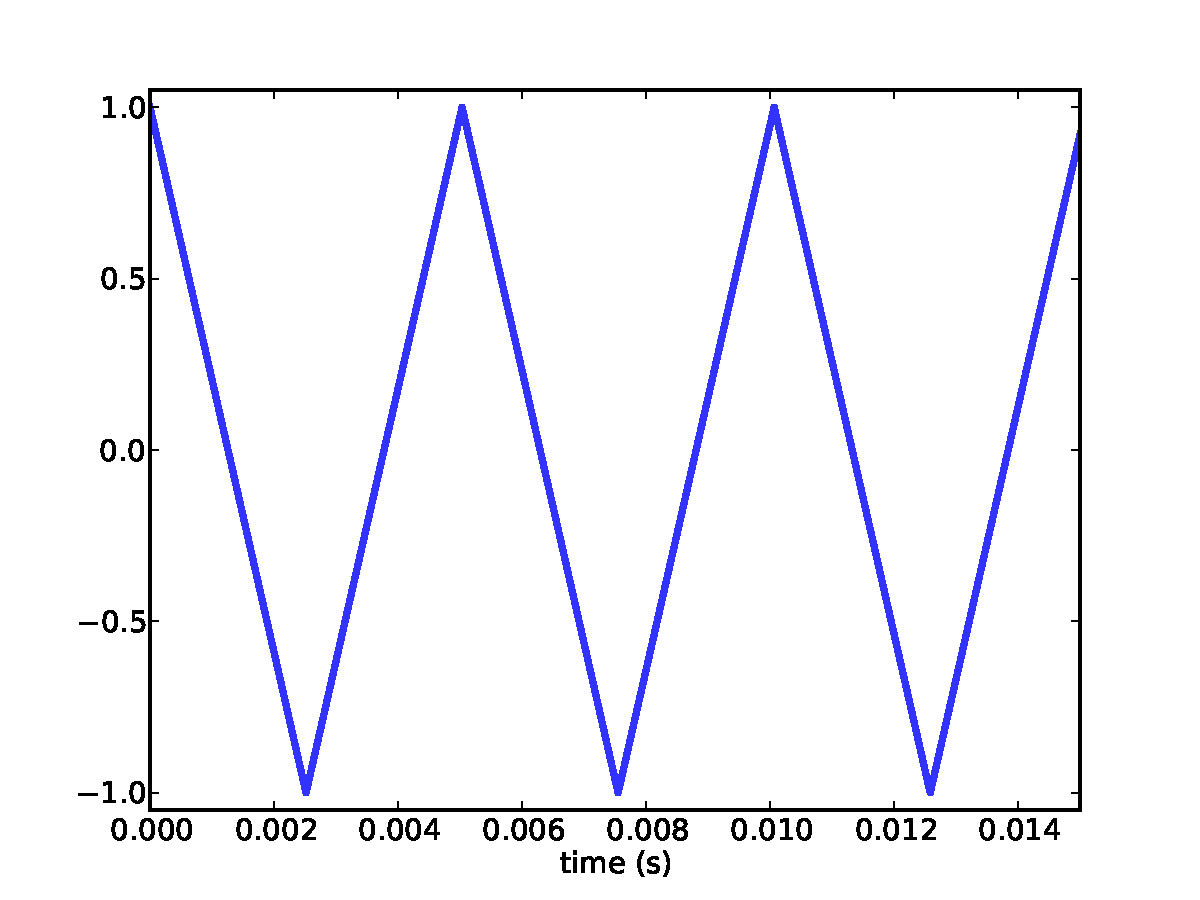
\includegraphics[height=2.5in]{figs/triangle-200-1.pdf}}
\caption{Segment of a triangle signal at 200 Hz.}
\label{fig.triangle.200.1}
\end{figure}

The triangle waveform is like a straight-line version of a sinusoid.
Figure~\ref{fig.triangle.200.1} shows a triangle waveform with
frequency 200 Hz.

To generate a triangle wave, you can use {\tt thinkdsp.TriangleSignal}:

\begin{verbatim}
class TriangleSignal(Sinusoid):
    
    def evaluate(self, ts):
        cycles = self.freq * ts + self.offset / PI2
        frac, _ = numpy.modf(cycles)
        ys = numpy.abs(frac - 0.5)
        ys = normalize(unbias(ys), self.amp)
        return ys
\end{verbatim}

{\tt TriangleSignal} inherits \verb"__init__" from {\tt Sinusoid},
so it takes the same arguments: {\tt freq}, {\tt amp}, and {\tt offset}.

The only difference is {\tt evaluate}.  As we saw before,
{\tt ts} is the sequence of sample times where we want to
evaluate the signal.

There are lots of ways to generate a triangle wave.  The details
are not important, but here's how {\tt evaluate} works:

\begin{enumerate}

\item {\tt cycles} is the number of cycles since the start time.
{\tt numpy.modf} splits the number of cycles into the fraction
part, stored in {\tt frac}, and the integer part, which is ignored.
\footnote{Using an underscore as a variable name is a convention that
means, ``I don't intend to use this value.''}

\item {\tt frac} is a sequence that ramps from 0 to 1 with the given
frequency.  Subtracting
0.5 yields values between -0.5 and 0.5.  Taking the absolute value
yields a waveform that zig-zags between 0.5 and 0.

\item {\tt unbias} shifts the waveform down so it is centered at 0, then
{\tt normalize} scales it to the given amplitude, {\tt amp}.

\end{enumerate}

Here's the code that generates Figure~\ref{fig.triangle.200.1}:

\begin{verbatim}
    signal = thinkdsp.TriangleSignal(200)
    duration = signal.period*3
    segment = signal.make_wave(duration, framerate=10000)
    segment.plot()
\end{verbatim}


\section{Harmonics}

Next we can compute the spectrum of this waveform:

\begin{verbatim}
    wave = signal.make_wave(duration=0.5, framerate=framerate)
    spectrum = wave.make_spectrum()
    spectrum.plot()
\end{verbatim}

\begin{figure}
% example2.py
\centerline{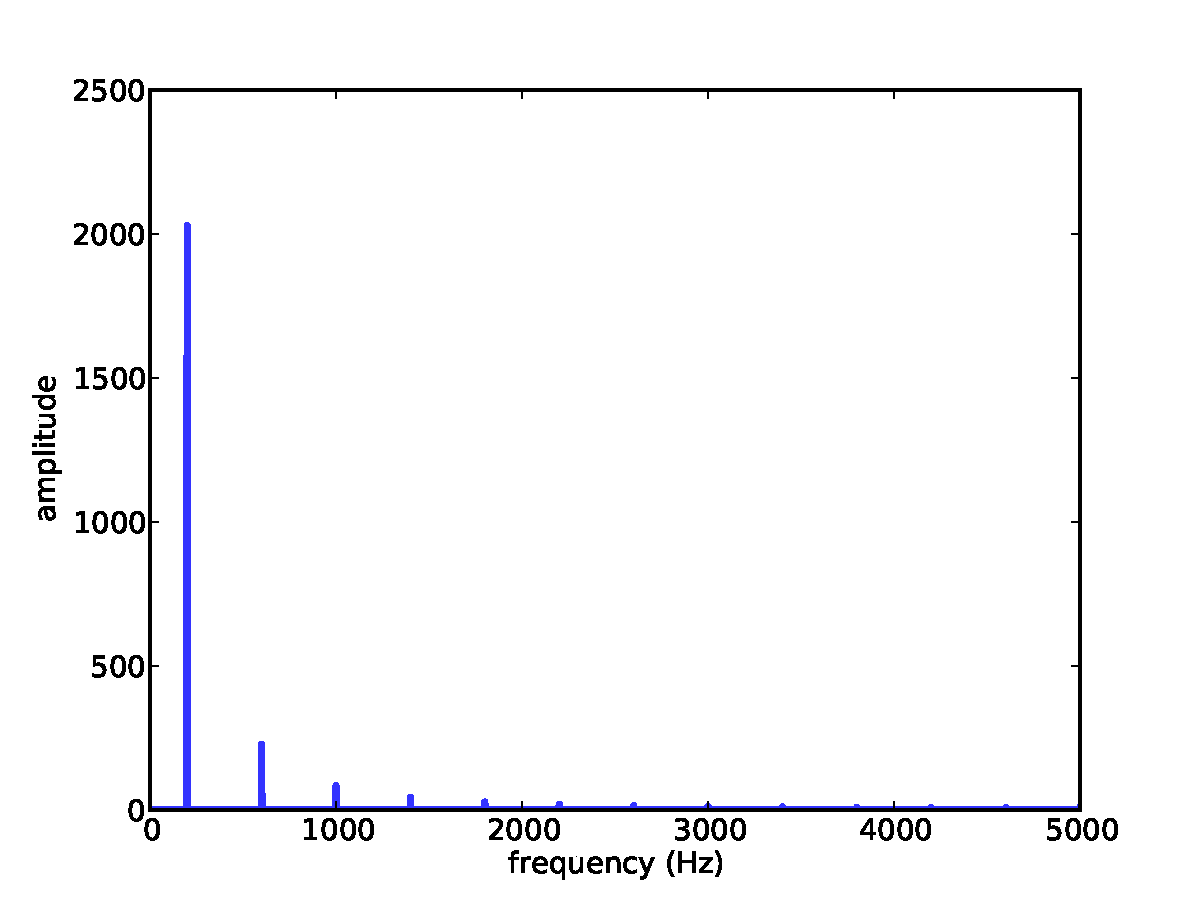
\includegraphics[height=2.5in]{figs/triangle-200-2.pdf}}
\caption{Spectrum of a triangle signal at 200 Hz.}
\label{fig.triangle.200.2}
\end{figure}

Figure~\ref{fig.triangle.200.2} shows the result.  As expected, the
highest peak is at the fundamental frequency, 200 Hz, and there
are additional peaks at harmonic frequencies, which are integer
multiples of 200.

But one surprise is that there are no peaks at the even multiples:
400, 800, etc.  The harmonics of a triangle wave are all
odd multiples of the fundamental frequency, in this example
600, 1000, 1400, etc.

Another feature of this spectrum is the relationship between the
amplitude and frequency of the harmonics.  The amplitude of the
harmonics drops off in proportion to frequency squared.  For example
the frequency ratio of the first two harmonics (200 and 600 Hz) is 3, and the
amplitude ration is approximately 9.  The frequency ratio of the
next two harmonics (600 and 1000 Hz) is 1.7, and the amplitude ratio
is approximately $1.7^2 = 2.9$.

{\tt thinkdsp} also provides {\tt SquareSignal}, which represents
a square signal.  Here's the class definition:

\begin{verbatim}
class SquareSignal(Sinusoid):
    
    def evaluate(self, ts):
        cycles = self.freq * ts + self.offset / PI2
        frac, _ = numpy.modf(cycles)
        ys = self.amp * numpy.sign(unbias(frac))
        return ys
\end{verbatim}

Like {\tt TriangleSignal}, {\tt SquareSignal} inherits 
\verb"__init__" from {\tt Sinusoid}, so it takes the same
parameters.

And the {\tt evaluate} method is similar.  Again, {\tt cycles} is
the number of cycles since the start time, and {\tt frac} is the
fractional part, which ramps from 0 to 1 each period.

{\tt unbias} shifts {\tt frac} so it ramps from -0.5 to 0.5,
then {\tt numpy.sign} maps the negative values to -1 and the
positive values to 1.  Multiplying by {\tt amp} yields a square
wave that jumps between {\tt -amp} and {\tt amp}.

\begin{figure}
% example2.py
\centerline{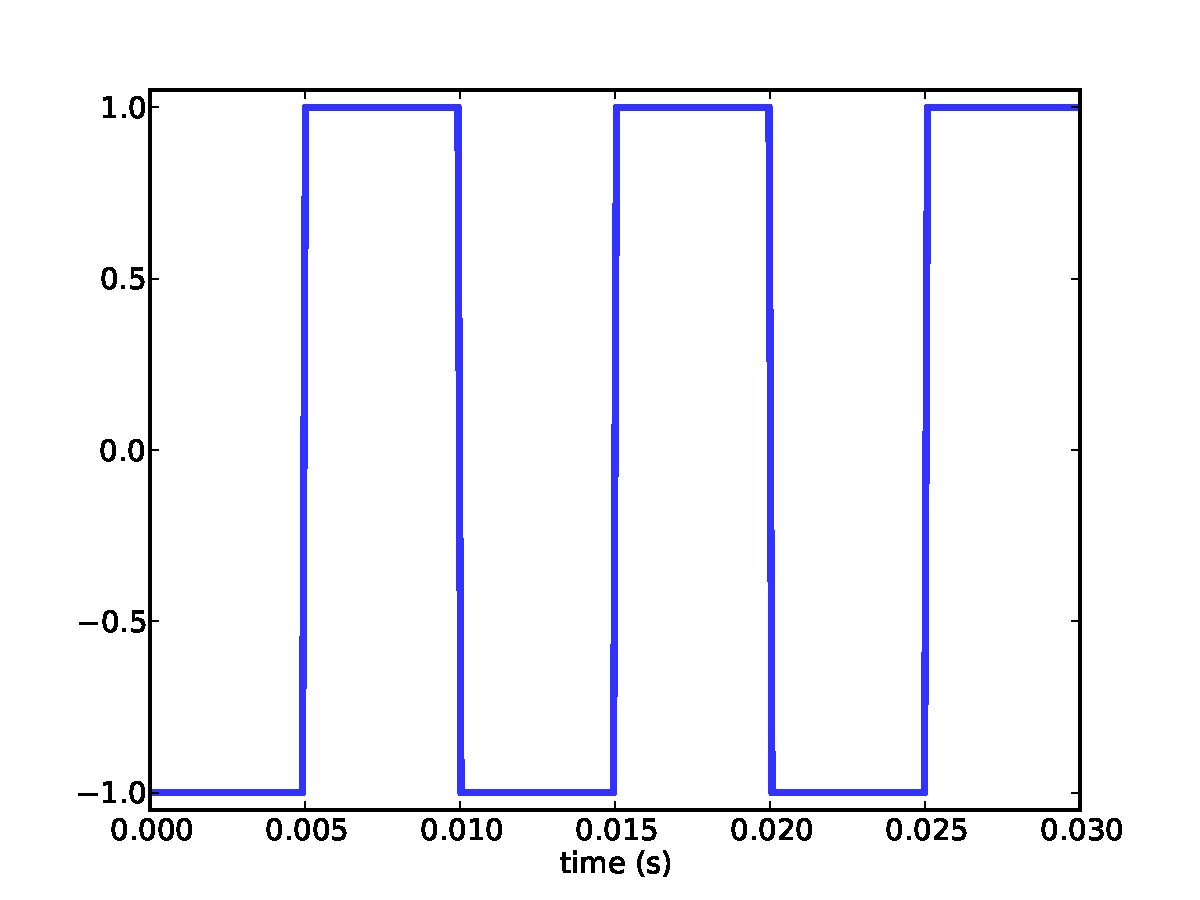
\includegraphics[height=2.5in]{figs/square-100-1.pdf}}
\caption{Segment of a square signal at 100 Hz.}
\label{fig.square.100.1}
\end{figure}

\begin{figure}
% example2.py
\centerline{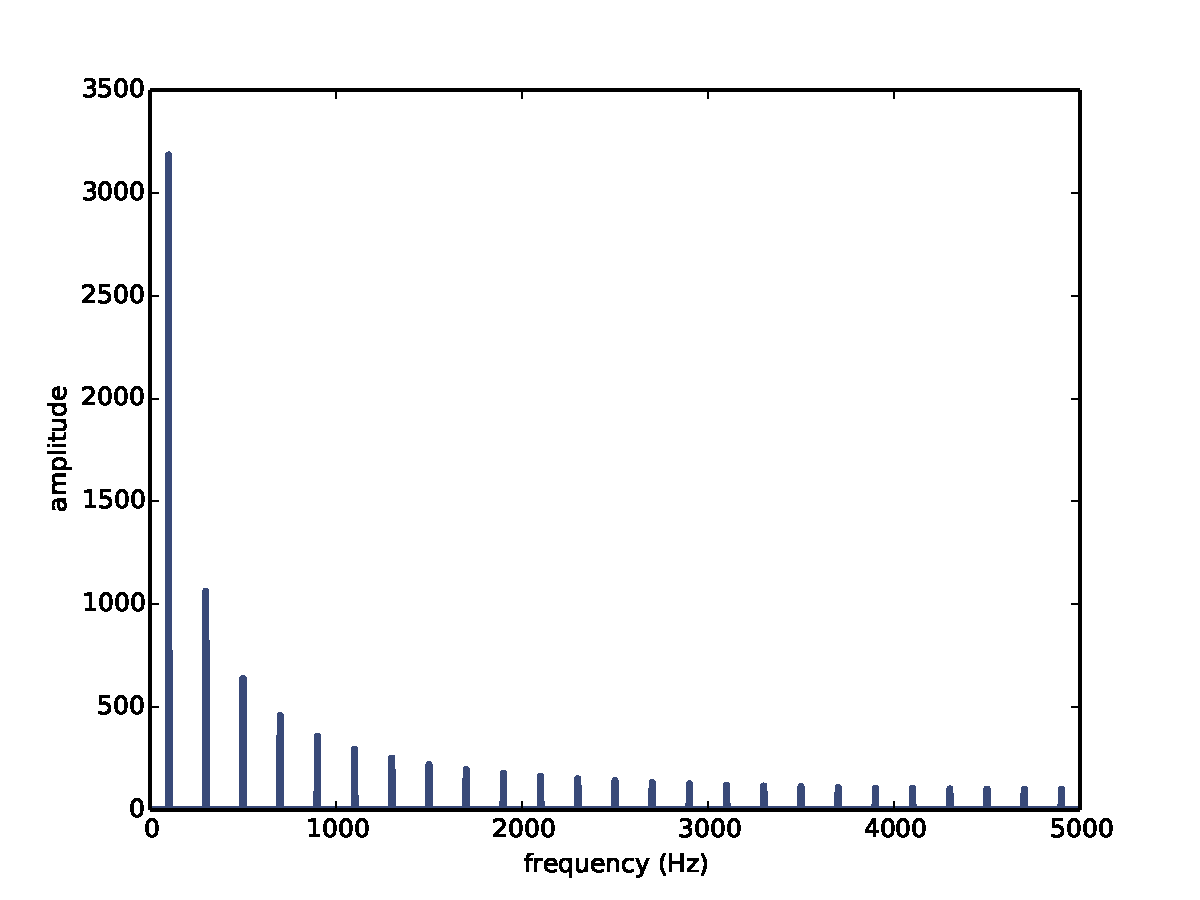
\includegraphics[height=2.5in]{figs/square-100-2.pdf}}
\caption{Spectrum of a square signal at 100 Hz.}
\label{fig.square.100.2}
\end{figure}

Figure~\ref{fig.square.100.1} shows three periods of a square
wave with frequency 100 Hz,
and Figure~\ref{fig.square.100.2} shows its spectrum.

Like a triangle wave, the square wave contains only odd harmonics,
which is why there are peaks at 300, 500, and 700 Hz, etc.
But the amplitude of the harmonics drops off more slowly.
Specifically, amplitude drops in proportion to frequency (not frequency
squared).


\section{Aliasing}

\begin{figure}
% example2.py
\centerline{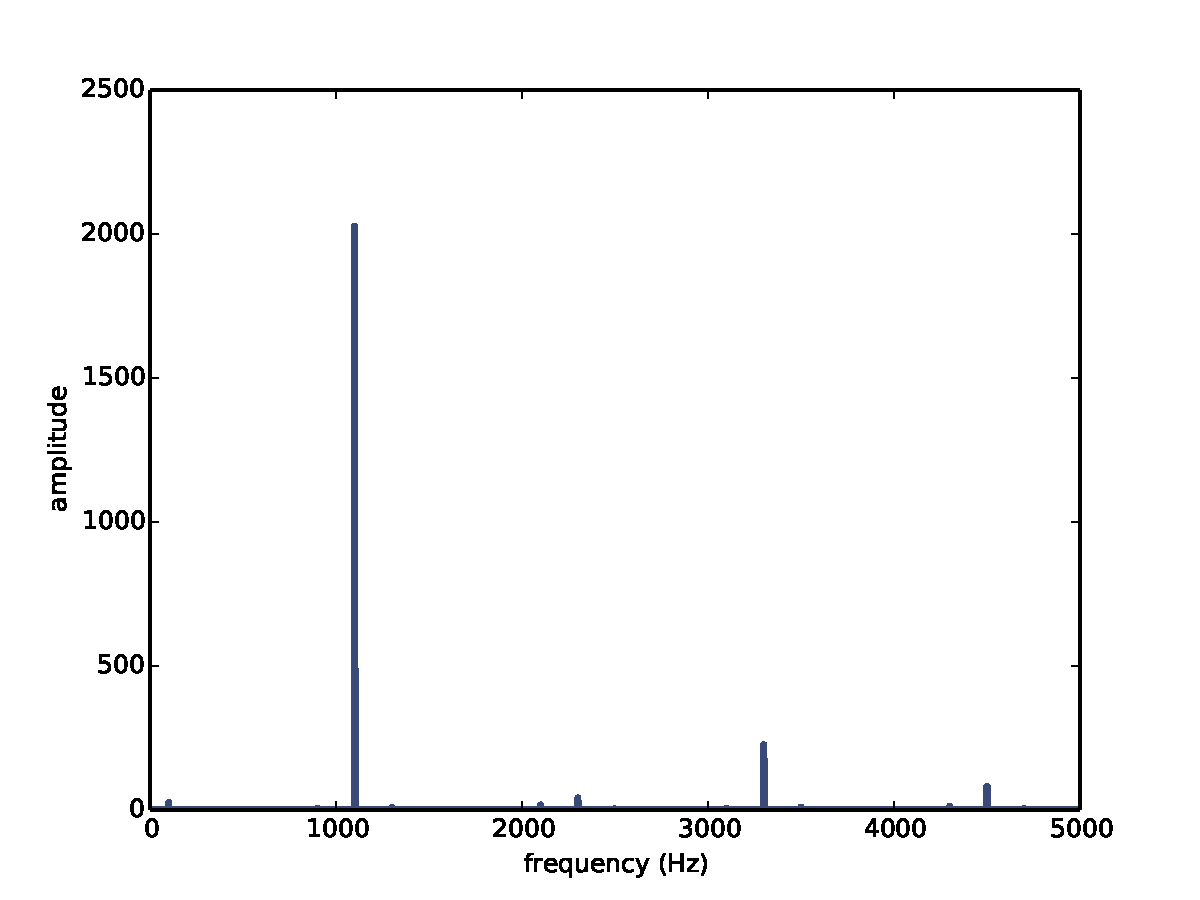
\includegraphics[height=2.5in]{figs/triangle-1100-2.pdf}}
\caption{Spectrum of a triangle signal at 1100 Hz sampled at
10,000 frames per second.}
\label{fig.triangle.1100.2}
\end{figure}

I have a confession.  I chose the examples in the previous section
carefully,
to avoid showing you something confusing.  But now it's time to get
confused.

Figure~\ref{fig.triangle.1100.2} shows the spectrum of a triangle wave at 1100 Hz, sampled
at 10,000 frames per second.

As expected, there are peaks at 1100 and 3300 Hz, but the third
peak is at 4500, not 5500 Hz as expected.  There is a small fourth peak
at 2300, not 7700 Hz.  And if you look very closely, the peak that should
be at 9900 is actually at 100 Hz.  What's going on?

The fundamental problem is that when you evaluate the signal at
discrete points in time, you lose information about what happens
between samples.  For low frequency components, that's not a
problem, because you have lots of samples per period.

But if you sample a signal at 5000 Hz with 10,000 frames per second,
you only have two samples per period.  That's enough to measure the
frequency (it turns out), but it doesn't tell you much about
the shape of the signal.

If the frequency is higher, like the 5500 Hz component of the
triangle wave, things are worse: you don't even get the
frequency right.

To see why, let's generate cosine signals at 4500 and 5500 Hz,
and sample them at 10,000 frames per second:

\begin{verbatim}
    framerate = 10000

    signal = thinkdsp.CosSignal(4500)
    duration = signal.period*5
    segment = signal.make_wave(duration, framerate=framerate)
    segment.plot()

    signal = thinkdsp.CosSignal(5500)
    segment = signal.make_wave(duration, framerate=framerate)
    segment.plot()
\end{verbatim}

\begin{figure}
% example2.py
\centerline{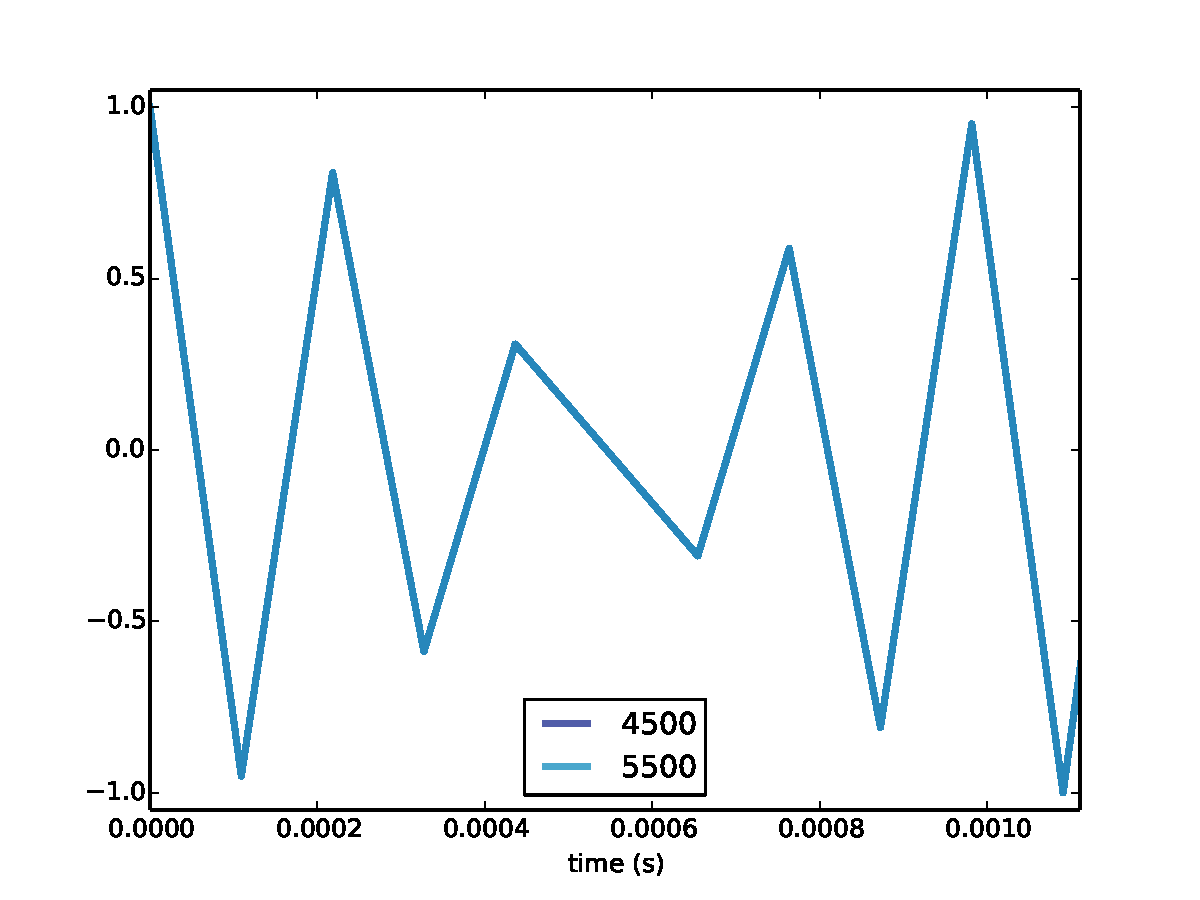
\includegraphics[height=2.5in]{figs/aliasing-3.pdf}}
\caption{Cosine signals at 4500 and 5500 Hz, sampled at 10,000 frames
per second.}
\label{fig.aliasing-3}
\end{figure}

Figure~\ref{fig.aliasing-3} shows the result.  The
sampled waveform doesn't look very much like a sinusoid, but the
bigger problem is that the two waveforms are exactly the same!

When we sample a 5500 Hz signal at 10,000 frames per second, the
result is indistinguishable from a 4500 Hz signal.

For the same reason, a 7700 Hz signal is indistinguishable
from 2300 Hz, and a 9900 Hz is indistinguishable from 100 Hz.

This effect is called {\bf aliasing} because when the high frequency
signal is sampled, it disguises itself as a low frequency signal.

In this example, the highest frequency we can measure is 5000 Hz,
which is half the sampling rate.  Frequencies above 5000 Hz are folded
back below 5000 Hz, which is why this threshold is sometimes called
the ``folding frequency,'' but more often it is called the {\bf
  Nyquist frequency}.  See
\url{http://en.wikipedia.org/wiki/Nyquist_frequency}.

The folding pattern continues if the aliased frequency goes below
zero.  For example, the 5th harmonic of the 1100 Hz triangle wave is
at 12,100 Hz.  Folded at 5000 Hz, it would appear at -2100 Hz, but it
gets folded again at 0 Hz, back to 2100 Hz.  In fact, you can see a
small peak at 2100 Hz in Figure~\ref{fig.square.100.2}, and the next
one at 4300 Hz.


\section{Exercises}

\begin{exercise}
Listen to the various non-sinusoidal waveforms.
\end{exercise}

\begin{exercise}
Start with a sawtooth.  Compute the DFT.  Remove all harmonics above
the $i$th.
Compute the inverse DFT and see what it looks like.
Repeat for a range of values of $i$.
\end{exercise}

\begin{exercise}
Write a new Signal type, compute it's DFT and listen to it.  What
happens if the signal is discontinuous?  What if the signal is continuous
but the slope is discontinuous?
\end{exercise}

\begin{exercise}
Make a frequency-limited sawtooth wave and see what it looks like
and sounds like.
See \url{http://en.wikipedia.org/wiki/Sawtooth_wave}.

\begin{exercise}
What does a square wave sound like underwater?
\end{exercise}

\begin{exercise}
Sample an 1100 Hz triangle at 10000 frames per second and listen to it.
Can you hear the aliased harmonic?  Might help to play a sequence of
notes with increasing pitch.
\end{exercise}

\begin{exercise}
Compute the spectrum of an 1100 Hz square wave.
\end{exercise}


\end{exercise}


\chapter{Non-periodic signals}


\section{Chirp}

The signals we have worked with so far are periodic, which means
that they repeat forever.  It also means that their spectrums do
no vary in time.  In this chapter, we consider non-periodic signals,
which includes any signal whose frequency components change over time.
In other words, pretty much all sound signals.

We'll start with a {\bf chirp}, which is a signal with variable
frequency.  Here is a class that represents a chirp:

\begin{verbatim}
class Chirp(Signal):
    
    def __init__(self, start=440, end=880, amp=1.0):
        self.start = start
        self.end = end
        self.amp = amp
\end{verbatim}

{\tt start} and {\tt end} are the frequencies, in Hz, at the start
and end of the chirp.  {\tt amp} is amplitude.

In a linear chirp, the frequency increases linearly from {\tt start}
to {\tt end}.  Here is the function that evaluates the signal:

\begin{verbatim}
    def evaluate(self, ts):
        freqs = numpy.linspace(self.start, self.end, len(ts)-1)
        return self._evaluate(ts, freqs)
\end{verbatim}

{\tt ts} is the sequence of points in time where the signal should
be evaluated.  If the length of {\tt ts} is $n$, you can think of
it as a sequence of $n-1$ segments of time.  To compute the frequency
during each segment, we use {\tt numpy.linspace}.

\verb"_evaluate" is a helper function that does the rest of the
math:\footnote{Beginning a method name with an underscore makes it
``private,'' indicating that it is not part of the API that should
be used outside the class definition.}

\begin{verbatim}
    def _evaluate(self, ts, freqs):
        dts = numpy.diff(ts)
        dps = PI2 * freqs * dts
        phases = numpy.cumsum(dps)
        ys = self.amp * numpy.cos(phases)
        return ys
\end{verbatim}

{\tt numpy.diff} computes the difference between adjacent elements
of {\tt ts}, returning the length of each segment in seconds.  In
the usual case where the elements of {\tt ts} are equally spaced,
the {\tt dts} are all the same.

The next step is to figure out how much the phase changes during
each segment.  Since we know the frequency and duration of each
segment, the {\em change} in phase during each integral is
{\tt PI2 * freqs * dts}.

Given the changes in phase, {\tt numpy.cumsum} computes the total
phase at the end of each segment.  Finally {\tt numpy.cos}
maps from phase to amplitude.

It might not be obvious how this function works, so here's another
way to think about it.  When $f$ is constant, phase increases linearly
over time.  Mathematically:

\[ \phi = 2 \pi f t \]

If $f$ varies in time, we can find the relationship between phase
and the instantaneous value of $f$ by taking the time derivative
of both sides:

\[ \frac{d\phi}{dt} = 2 \pi f \]

In other words, frequency is the derivative of phase.  Or equivalently,
phase is the integral of frequency.  We can write the same
equation in differential form:

\[ d\phi = 2 \pi f dt \]

which looks a whole lot like this line from \verb"_evaluate":

\begin{verbatim}
        dps = PI2 * freqs * dts
\end{verbatim}

To find the total phase, you can imagine adding up the elements of
{\tt dps}, or if you like calculus, you can think of it as a
numerical solution of an integral.

Here's the code that creates and plays a chirp from 220 to 880 Hz, which
is two octaves from A3 to A5:

\begin{verbatim}
    signal = thinkdsp.Chirp(start=220, end=880)
    wave1 = signal.make_wave(duration=2)

    filename = 'chirp.wav'
    wave1.write(filename)
    thinkdsp.play_wave(filename)
\end{verbatim}

Before you go on, run this code and listen.


\section{Exponential chirp}

When you listen to this chirp, you might notice that the pitch
rises quickly at first and then slows down.
The chirp spans two octaves, but it only takes 2/3 s to span
the first octave, and twice as long to span the second.  

The reason is that our perception of pitch depends on the
logarithm of frequency.  As a result, the {\bf interval} we hear between
two notes depends on the {\em ratio} of their frequencies, not
the difference.  ``Interval'' is the musical term for the
perceived difference between two pitches.

For example, an octave is an interval where the ratio of two
pitches is 2.  So the interval from 220 to 440 is one octave
and the interval from 440 to 880 is also one octave.  The difference
in frequency is bigger, but the ratio is the same.

As a result, if frequency increases linearly, as in a linear
chirp, the perceived pitch increases logarithmically.

If you want the perceived pitch to increase linearly, the frequency
has to increase exponentially.  A signal with that shape is called
an {\bf exponential chirp}.

Here's the code that makes one:

\begin{verbatim}
class ExpoChirp(Chirp):
    
    def evaluate(self, ts):
        start, end = math.log10(self.start), math.log10(self.end)
        freqs = numpy.logspace(start, end, len(ts)-1)
        return self._evaluate(ts, freqs)
\end{verbatim}

Instead of {\tt numpy.linspace}, this version of evaluate uses
{\tt numpy.logspace}, which creates a series of frequencies
whose logarithms are equally spaced, which means that they increase
exponentially.

That's it; everything else is the same as Chirp.  Here's the code
that makes one:

\begin{verbatim}
    signal = thinkdsp.ExpoChirp(start=220, end=880)
    wave1 = signal.make_wave(duration=2)

    filename = 'expo_chirp.wav'
    wave1.write(filename)
    thinkdsp.play_wave(filename)
\end{verbatim}

Run this code and listen.  If you have a musical ear, this might
sound more like music than the linear chirp.


\section{Leakage}

\begin{figure}
% example3.py
\centerline{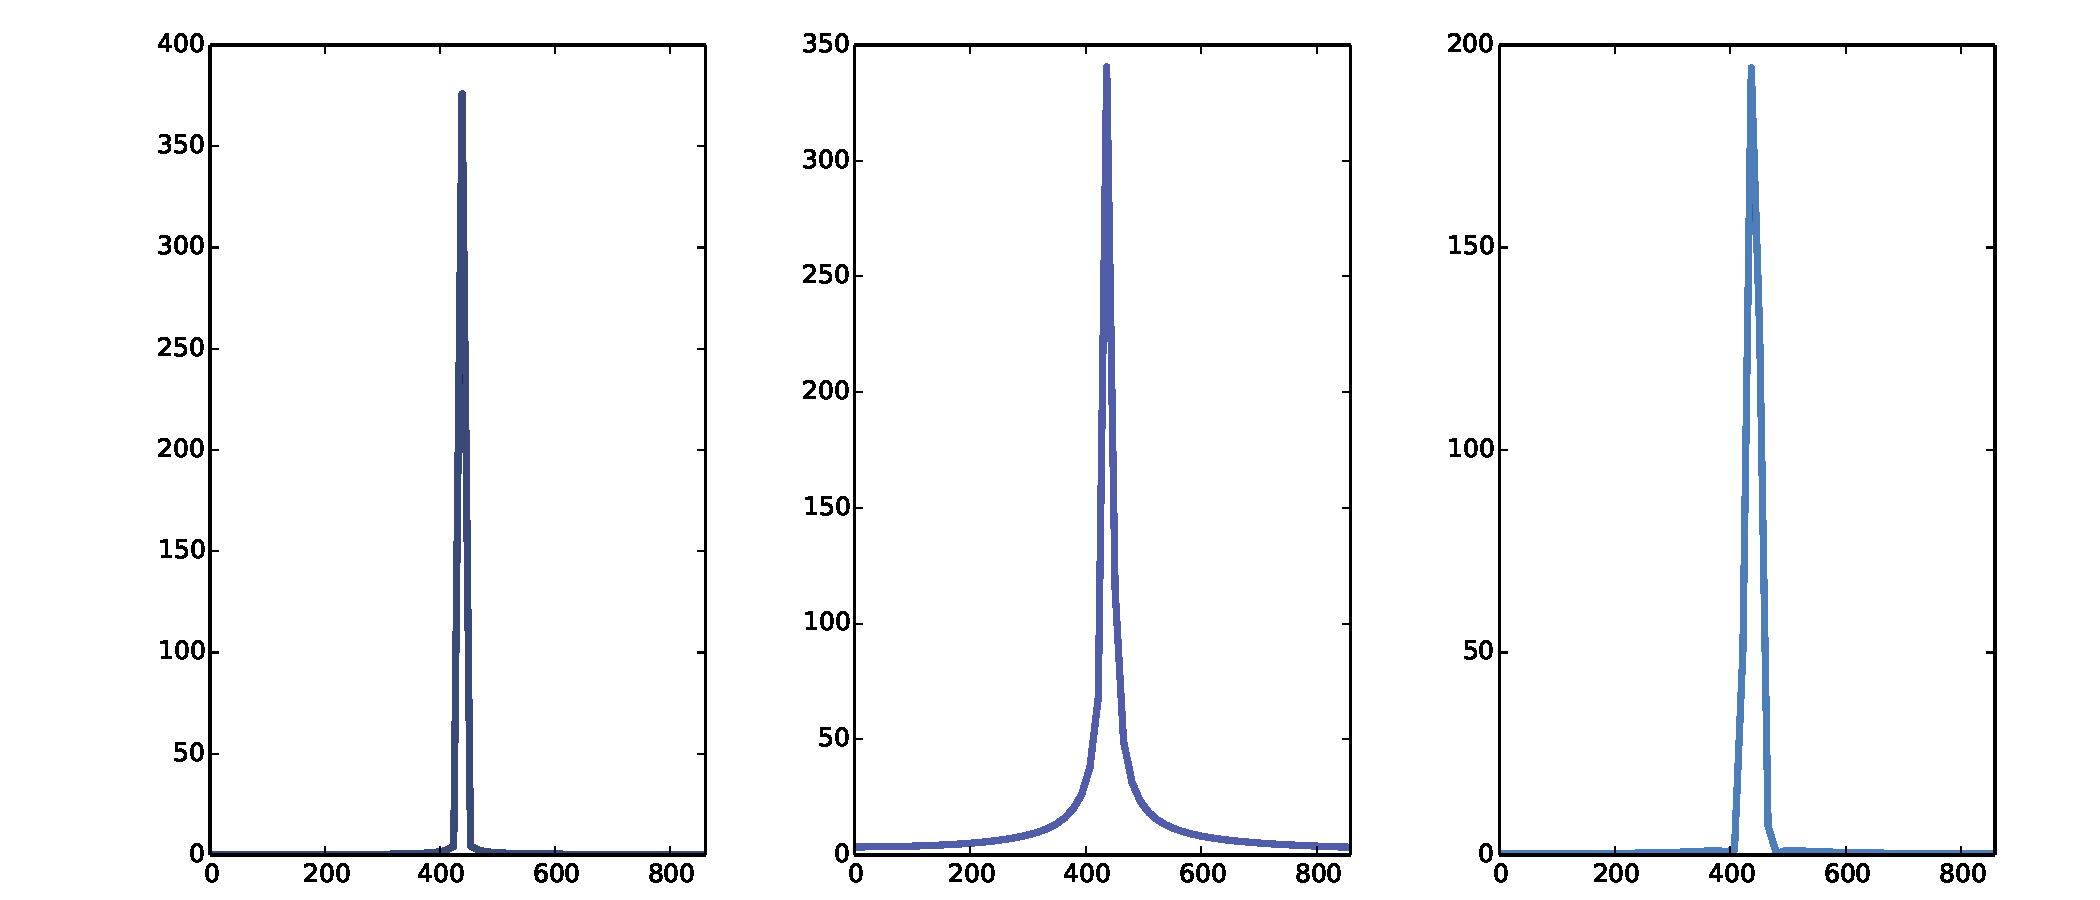
\includegraphics[height=2.5in]{figs/windowing1.pdf}}
\caption{Spectrum of (a) a periodic segment of a sinusoid, (b)
a non-periodic segment, (c) a tapered non-periodic segment.}
\label{fig.windowing1}
\end{figure}

In previous chapters, we used FFT to compute the spectrum of a wave.
Later, when we discuss how FFT works, we will learn that the algorithm
is based on the assumption that the signal is periodic.  In theory, we
should not use FFT on non-periodic signals, but in practice it happens
all the time.  But there are a few things you have to be careful about.

One common problem is dealing with discontinuities at the beginning
and end of a segment.  Because FFT assumes that the signal is periodic,
in a sense it connects the end of the segment back to the beginning
to make a loop.  If the end does not connect smoothly to the beginning,
the discontinuity creates additional frequency components in the
segment that are not in the signal.

As an example, let's start with a sine wave that contains only
one frequency component at 440 Hz.

\begin{verbatim}
    signal = thinkdsp.SinSignal(freq=440)
\end{verbatim}

If we select a segment that happens to be an integer multiple of
the period, the end of the segment connects smoothly with the
beginning, and FFT behaves well.

\begin{verbatim}
    duration = signal.period * 30
    wave = signal.make_wave(duration)
    spectrum = wave.make_spectrum()
\end{verbatim}

Figure~\ref{fig.windowing1}a shows the result.  As expected, there is
a single peak at 440 Hz.  But if the duration is not a multiple of the
period, bad things happen.  With {\tt duration = signal.period *
  30.25}, the signal starts at 0 and ends at 1.
Figure~\ref{fig.windowing1}b shows the spectrum of this segment.
Again, the peak is at 440 Hz, but now there are additional components
spread out from 240 to 640 Hz.  This spread is called ``spectral
leakage'', because some of the energy at the fundamental frequency
leaks into other frequencies.

In this case leakage happens because we are using FFT on a segment
that is not periodic.


\section{Windowing}

\begin{figure}
% example3.py
\centerline{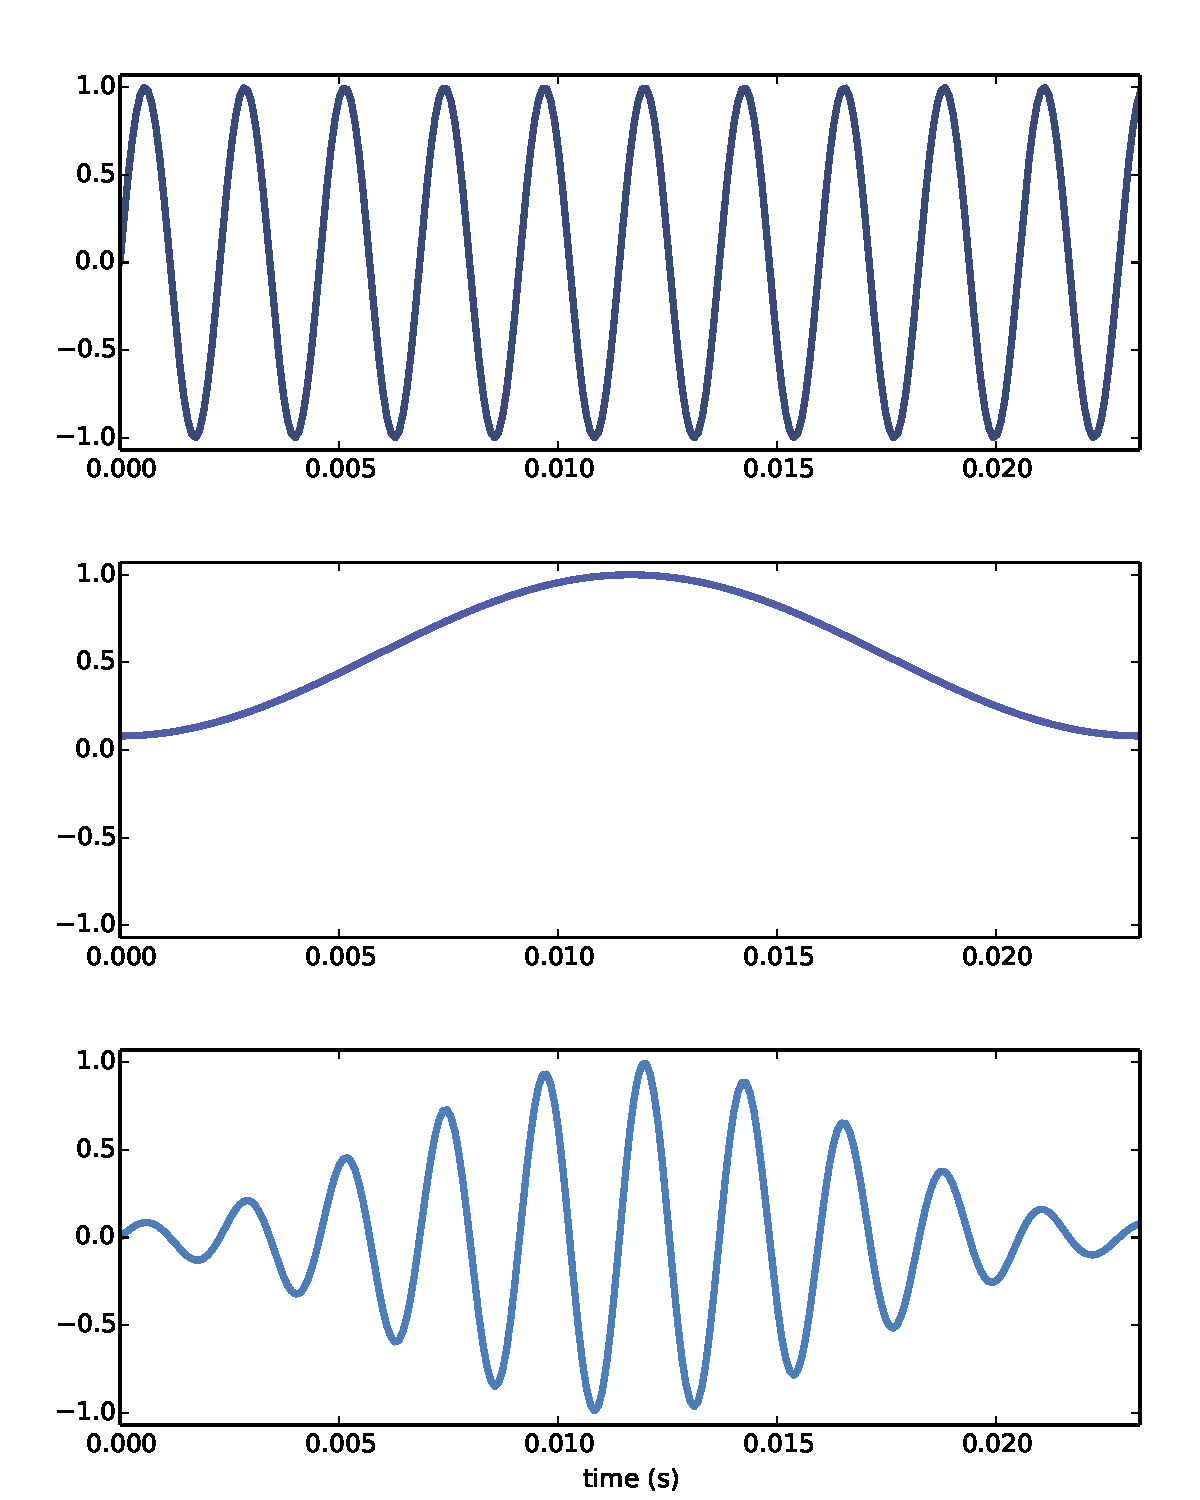
\includegraphics[height=2.5in]{figs/windowing2.pdf}}
\caption{(a) Segment of a sinusoid, (b) Hamming window, (c) product
of the segment and the window.}
\label{fig.windowing2}
\end{figure}

We can reduce leakage by smoothing out the discontinuity between
the beginning and end of the segment, and one way to do that is
{\bf windowing}.

A ``window'' is a function designed to transform a non-periodic
segment into something that can pass for periodic.
Figure~\ref{fig.windowing2}a shows a segment where the end does not
connect smoothly to the beginning.

Figure~\ref{fig.windowing2}b shows a ``Hamming window'', one of the
more common window functions.  No window function is perfect, but some
can be shown to be optimal for different applications.

Figure~\ref{fig.windowing2}c shows the result of multiplying the
window by the original signal.  Where the window is close to 1, the
signal is unchanged.  Where the window is close to 0, the signal is
attenuated.  Because the window tapers at both ends, the end of the
segment connects smoothly to the beginning.

Figure~\ref{fig.windowing1}c shows the spectrum of the tapered signal.
Windowing has reduced leakage substantially, but not completely. 

Here's what the code looks like.  {\tt Wave} provides {\tt hamming},
which applies a Hamming window:

\begin{verbatim}
    def hamming(self):
        self.ys *= numpy.hamming(len(self.ys))
\end{verbatim}

{\tt numpy.hamming} computes the Hamming window with the given number
of elements.  {\tt numpy} provides functions to compute other window
functions, including {\tt bartlett}, {\tt blackman}, {\tt hanning},
and {\tt kaiser}.  One of the exercises at the end of this chapter
asks you to experiment with these other windows.


\section{Spectrum of a chirp}

\begin{figure}
% example3.py
\centerline{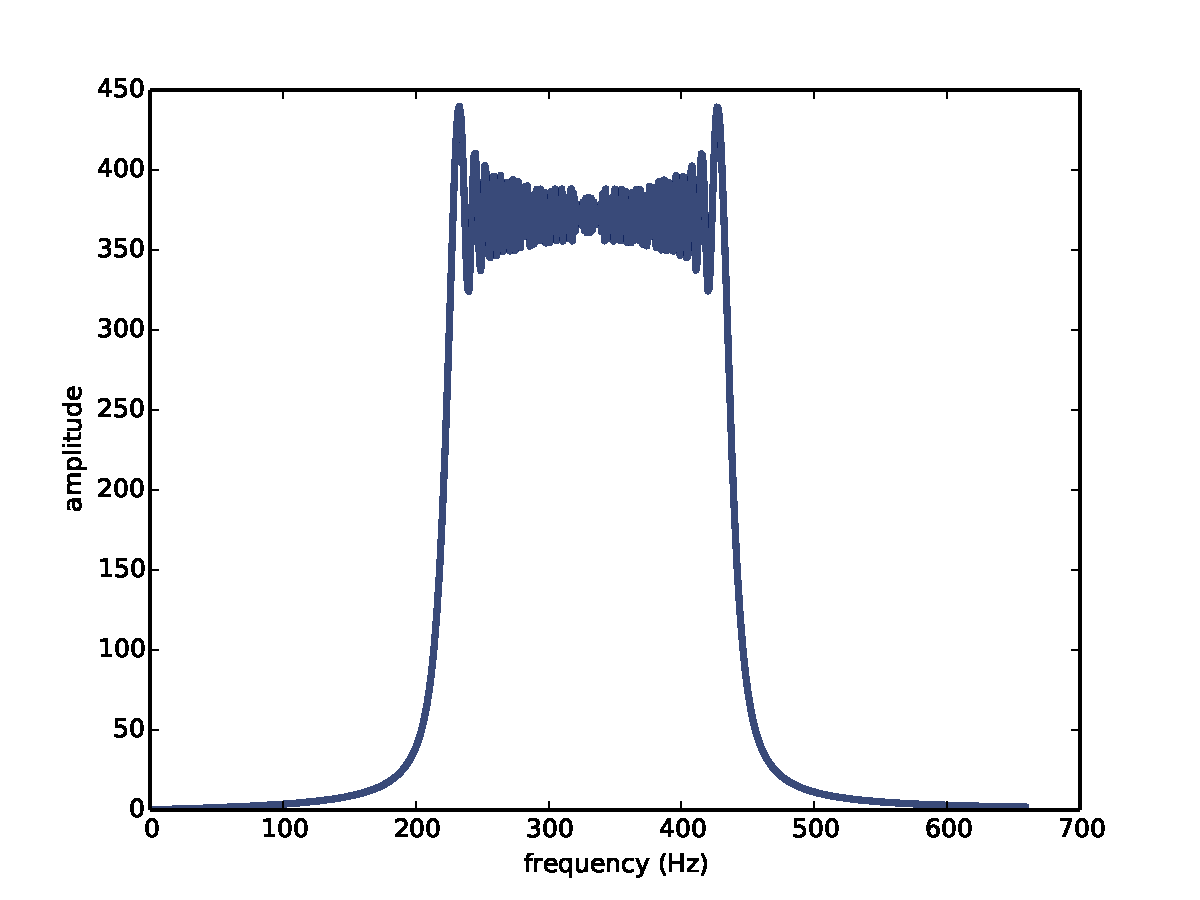
\includegraphics[height=2.5in]{figs/chirp1.pdf}}
\caption{Spectrum of a one-second one-octave chirp.}
\label{fig.chirp1}
\end{figure}

What do you think happens if you compute the spectrum of a chirp?
Here's an example that constructs a one-second one-octave chirp and
its spectrum:

\begin{verbatim}
    signal = thinkdsp.Chirp(start=220, end=440)
    wave = signal.make_wave(duration=1)
    spectrum = wave.make_spectrum()
\end{verbatim}

Figure~\ref{fig.chirp2} shows the result.  The spectrum shows
components at every frequency from 220 to 440 Hz with variations,
caused by leakage, that look a little like the Eye of Sauron.

The spectrum is approximately flat between 220 and 440 Hz, which
indicates that the signal spends equal time at each frequency in this
range.  Based on that observation, you should be able to guess what
the spectrum of an exponential chirp looks like.

The spectrum gives hints about the structure of the signal,
but it loses the relationship between frequency and time.
For example, we cannot tell by looking at this spectrum whether
the frequency went up or down, or both.


\section{Spectrogram}

\begin{figure}
% example3.py
\centerline{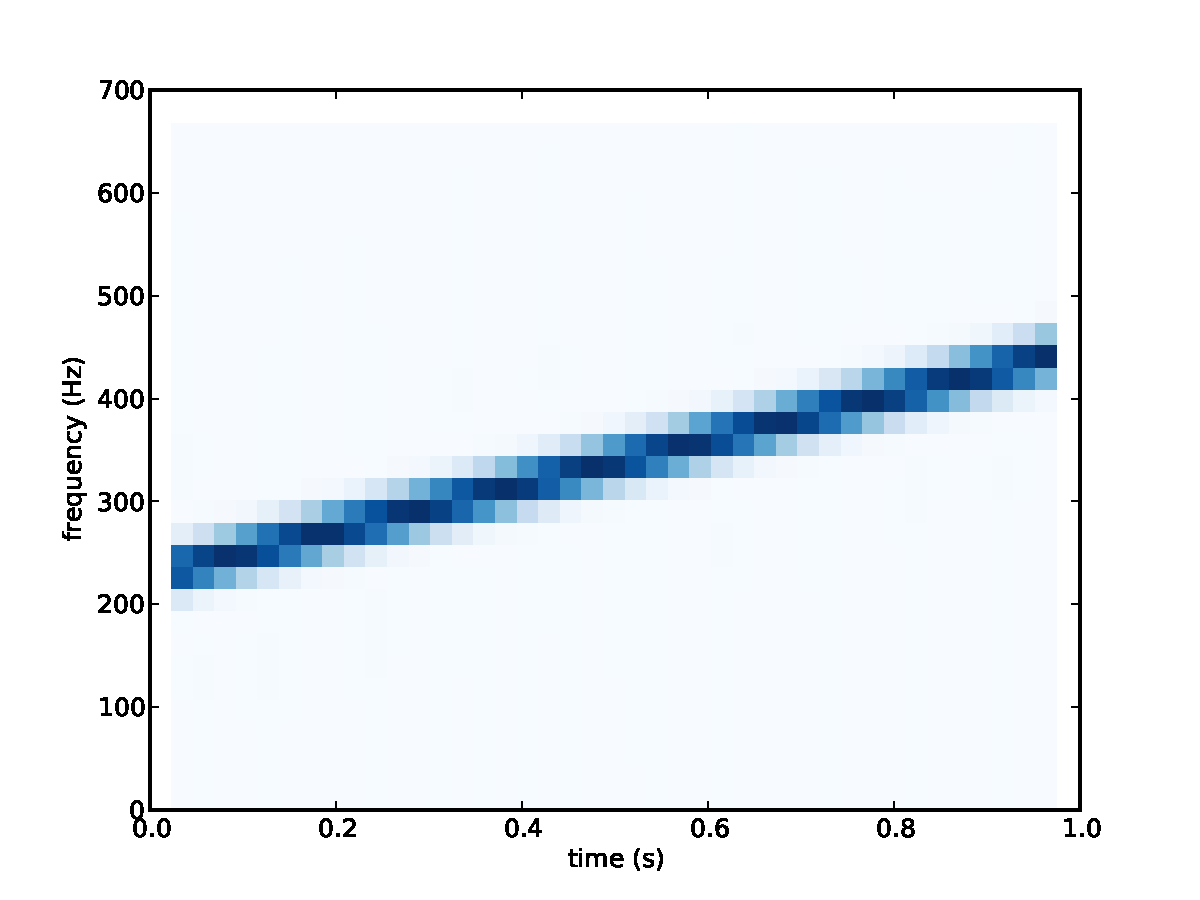
\includegraphics[height=2.5in]{figs/chirp2.pdf}}
\caption{Spectrogram of a one-second one-octave chirp.}
\label{fig.chirp2}
\end{figure}

To recover the relationship between frequency and time, we can break
the chirp into segments and plot the spectrum of each segment.  The
result is called a {\bf short-time Fourier transform} (STFT).

There are several ways to visualize a STFT, but the most common
is a {\bf spectrogram}, which shows time on the x-axis, and frequency
on the y-axis.  Each column in the spectrogram shows the spectrum of
a short segment, using color or grayscale to represent amplitude.

{\tt Wave} provides \verb"make_spectrogram", which returns a
{\tt Spectrogram} object:

\begin{verbatim}
    signal = thinkdsp.Chirp(start=220, end=440)
    wave = signal.make_wave(duration=1)
    spectrogram = wave.make_spectrogram(seg_length=512)
    spectrogram.plot(high=32)
\end{verbatim}

\verb"seg_length" is the number of samples in each segment.  I chose
512 because FFT is most efficient when the number of samples is a
power of 2.

Figure~\ref{fig.chirp2} shows the result.  The x-axis shows time from
0 to 1 seconds.  The y-axis shows frequency from 0 to 700 Hz.  I cut
off the top part of the spectrogram; the full range goes to 5012.5 Hz,
which is half of the framerate.

The spectrogram shows clearly that frequency increases linearly
over time.  Similarly, in the spectrogram of an exponential chirp, we
can see the shape of the exponential curve.

However, notice that the peak in each column is blurred across 2--3
cells.  This blurring reflects the limited resolution of the
spectrogram.


\section{The Gabor limit}

The {\bf time resolution} of the spectrogram is the duration of the
segments, which corresponds to the width of the cells in the
spectrogram.  Since each segment is 512 frames, and there are 11,025
frames per second, there are 0.046 seconds per segment.

The {\bf frequency resolution} is the frequency range between
components in the spectrum, which corresponds to the height of the
cells.  With 512 frames, we get 256 frequency components over a range
from 0 to 5012.5 Hz, so the range between components is 21.5 Hz.

More generally, if $n$ is the segment length, the spectrum contains
$n/2$ components.  If the framerate is $r$, the maximum frequency
in the spectrum is $r/2$.
So the time resolution is $n/r$ and the frequency resolution is 
$r/2$ divided by $n/2$, which is $r/n$.

Ideally we would like time resolution to be small, so we can see rapid
changes in frequency.  And we would like frequency resolution to be
small so we can see small changes in frequency.  But you can't have
both.  Notice that time resolution, $n/r$, is the inverse of frequency
resolution, $r/n$.  So if one gets smaller, the other gets bigger.

For example, if you double the segment length, you cut frequency
resolution in half (which is good), but you double time resolution
(which is bad).  Even increasing the framerate doesn't help.  You get
more samples to play with, but the range of frequencies increases at
the same time.

This tradeoff is called the ``Gabor limit'' and it is a fundamental
limitation of this kind of time-frequency analysis.


\section{Implementing spectrograms}

\begin{figure}
% example3.py
\centerline{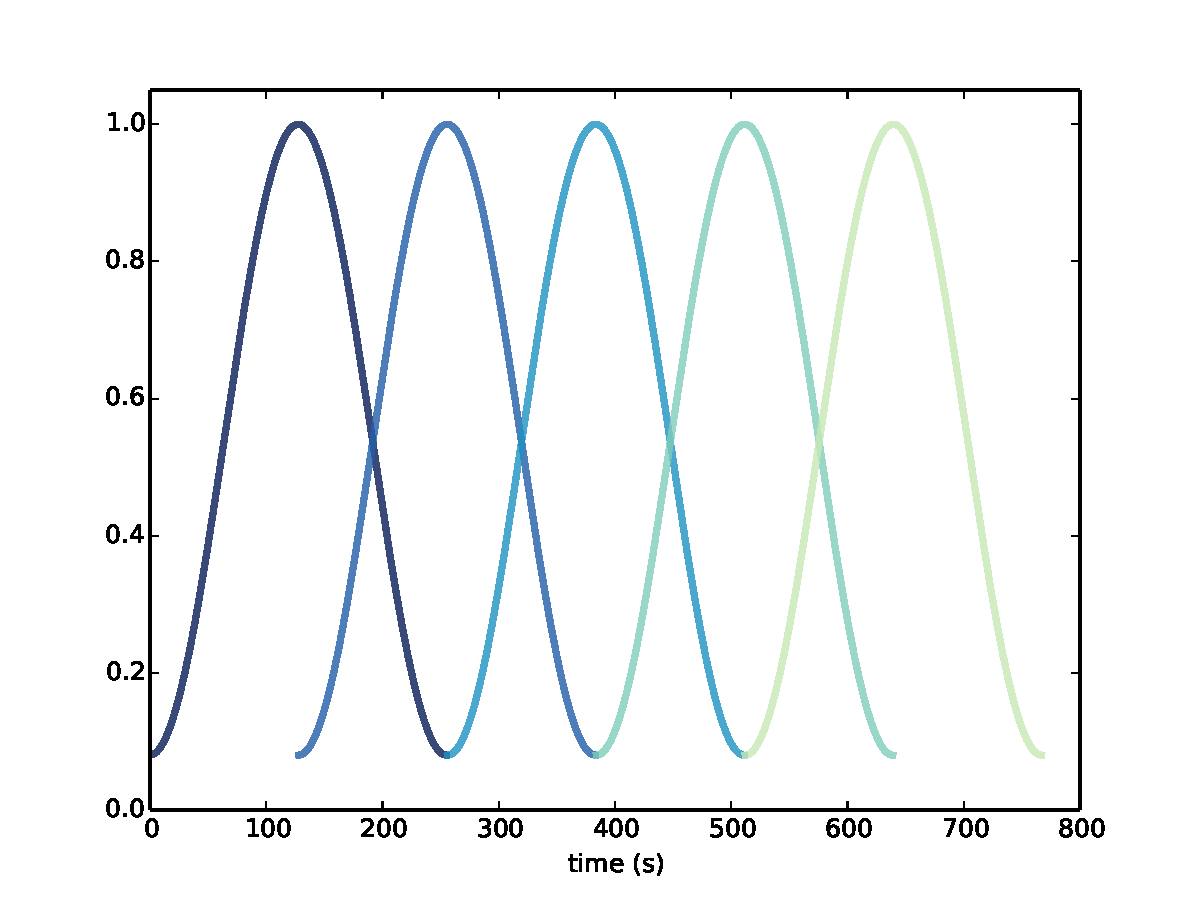
\includegraphics[height=2.5in]{figs/windowing3.pdf}}
\caption{Overlapping Hamming windows.}
\label{fig.windowing3}
\end{figure}

Here is the {\tt Wave} method that computes spectrograms:

\begin{verbatim}
    def make_spectrogram(self, seg_length):
        n = len(self.ys)
        window = numpy.hamming(seg_length)

        start, end, step = 0, seg_length, seg_length / 2
        spec_map = {}

        while end < n:
            ys = self.ys[start:end] * window
            hs = numpy.fft.rfft(ys)

            t = (start + end) / 2.0 / self.framerate
            spec_map[t] = Spectrum(hs, self.framerate)

            start += step
            end += step

        return Spectrogram(spec_map, seg_length, window_func)
\end{verbatim}

\verb"seg_length" is the number of samples in each segment.
{\tt n} is the number of samples in the wave.  {\tt window}
is a Hamming window with the same length as the segments.

{\tt start} and {\tt end} are the slice indices that select
the segments from the wave.  {\tt step} is the offset between
segments.  Since {\tt step} is half of \verb"seg_length", the
segments overlap by half.  Figure~\ref{fig.windowing3} shows what
these overlapping windows look like.

Inside the while loop, we select a slice from the wave, multiply
by the window, and compute the FFT.  Then we construct a Spectrum
object and add it to \verb"spec_map" which is a map from the
midpoint of the segment in time to the Spectrum object.

Finally, the method constructs and returns a Spectrogram.  Here
is the definition of Spectrogram:

\begin{verbatim}
    def __init__(self, spec_map, seg_length):
        self.spec_map = spec_map
        self.seg_length = seg_length
\end{verbatim}

And {\tt Spectrogram} provides {\tt plot}, which generates a
pseudocolor plot:

\begin{verbatim}
    def plot(self, low=0, high=None):
        ts = self.times()
        fs = self.frequencies()[low:high]

        # copy amplitude from each spectrum into a column of the array
        size = len(fs), len(ts)
        array = numpy.zeros(size, dtype=numpy.float)

        # copy each spectrum into a column of the array
        for i, t in enumerate(ts):
            spectrum = self.spec_map[t]
            array[:,i] = spectrum.amps[low:high]

        thinkplot.pcolor(ts, fs, array)
\end{verbatim}

{\tt plot} uses {\tt times}, which the returns the midpoint of each
time segment in a sorted sequence, and {\tt frequencies}, which returns
the frequencies of the components in the spectrums.

{\tt array} is a numpy array that holds the amplitudes from the
spectrums, with one column for each point in time and one row
for each frequency.  The {\tt for} loop iterates through the times
and copies each spectrum into a column of the array.

Finally {\tt thinkplot.color} is a wrapper around {\tt pyplot.pcolor},
which generates the pseudocolor plot.

So that's how Spectrograms are implemented.


\section{Exercises}

\begin{exercise}
Write a class called {\tt SawtoothChirp} that extends {\tt Chirp}
and overrides {\tt evaluate} to generate a sawtooth waveform with
frequency that increases (or decreases) linearly.

Hint: combine the evaluate functions from {\tt Chirp} and {\tt
  SawtoothSignal}.

Draw a sketch of what you think the spectrogram of this signal
looks like, and then plot it.  The effect of aliasing should be
visually apparent, and if you listen carefully, you can hear it.
\end{exercise}

\begin{exercise}
Another way to generate a sawtooth chirp is to add up a harmonic
series of sinusoidal chirps.  Write another version of {\tt
  SawtoothChirp} that uses this method and plot the histogram.

If you truncate the harmonic series at the Nyquist frequency, you
should be able to avoid aliasing.
\end{exercise}


\begin{exercise}
In musical terminology, a ``glissando'' is a note that slides from one
pitch to another, so it is similar to a chirp.  A trombone player can
play a glissando by extending the trombone slide while blowing
continuously.  As the slide extends, the total length of the tube gets
longer, and the resulting pitch is inversely proportional to length.

Write a function that simulates a trombone glissando from C4 up to F4
and back down to C4.  C3 is 262 Hz; F3 is 349 Hz.

Assuming that the player moves the slide at a constant speed, how
does frequency vary with time?  Is a trombone glissando more like
a linear or exponential chirp?
\end{exercise}


\begin{exercise}
Try other window functions.
\end{exercise}

\begin{exercise}
Make a spectrogram of the clarinet glissando at the beginning of
Rhapsody in Blue.

% http://archive.org/details/rhapblue11924
\end{exercise}

\begin{exercise}
Make a recording of a series of vowel sounds and look at the spectrogram.
Can you identify different vowels?
\end{exercise}

%\begin{exercise}
%Compute the inverse spectrogram of an image and listen to it.
%Landscape images might work best.
%\end{exercise}




\chapter{Pitch tracking}

\section{Spectrum of vowels}

\section{Spectrum of a piano}

\section{Music synthesis}

Additive synthesis.

Envelope generation.

\section{Convert music notation to a signal}

\section{Compute the spectrogram of an idealized performance}

\section{Compute the spectrogram of an actual performance}

\section{Pitch tracking algorithm}

\section{Pitch shifting}

Auto-tune?


\chapter{Spectral density estimation}

Spectrum of symbal crash, applause.

Synthesize white and pink noise.

Estimate the spectrum of a long time series (stock market data?
astronomical data?)

Welch's method, discussion of amplitude, amplitude density, power
and decibels.


\chapter{Discrete cosine transform}

The topic of the next two chapters is the {\bf Discrete Cosine
  Transform} (DCT), which is used in MP3 and related formats for
compressing music, JPEG and similar formats for images, and the MPEG
family of formats for video.

DCT is similar in many ways to the discrete Fourier transform (DFT).
Once we learn how DCT works, it will be easier to explain DFT.

Here are the steps we will follow to get there:

\begin{enumerate}

\item We'll start with the synthesis problem: given a set of frequency
  components and their amplitudes, how can we construct a waveform?

\item Next we'll rewrite the synthesis problem using numpy arrays.
  This move is good for performance, and also provides insight
  into the analysis problem.

\item Next we'll look at the analysis problem: given a signal and a
  set of frequencies, how can we find the amplitude of each frequency
  component?  We'll start with a solution that is conceptually simple
  but slow.

\item Finally, we'll use some principles from linear algebra to find a
  more efficient algorithm.  If you already know linear algebra,
  that's great, but I will explain what you need as we go.

\end{enumerate}

Let's get started.


\section{Synthesis}

Suppose I give you a list of amplitudes and a list of frequencies,
and ask you to construct a signal that is the sum of these frequency
components.  Using objects in the {\tt thinkdsp} module, there is
a simple way to perform this operation, which is called {\bf synthesis}:

\begin{verbatim}
def synthesize1(amps, freqs, ts):
    components = [thinkdsp.CosSignal(freq, amp)
                  for amp, freq in zip(amps, freqs)]
    signal = thinkdsp.SumSignal(*components)

    ys = signal.evaluate(ts)
    return ys
\end{verbatim}

{\tt amps} is a list of amplitudes, {\tt freqs} is the list
of frequencies, and {\tt ts} is the sequence
of times where the signal should be evaluated.

{\tt components} is a list of {\tt CosSignal} objects, one for
each amplitude-frequency pair.  {\tt SumSignal} represents the
sum of these frequency components.

Finally, {\tt evaluate} computes the value of the signal at each
time in {\tt ts}.

We can test this function like this:

\begin{verbatim}
    amps = numpy.array([0.6, 0.25, 0.1, 0.05])
    freqs = [100, 200, 300, 400]
    framerate = 11025

    ts = numpy.linspace(0, 1, framerate)
    ys = synthesize1(amps, freqs, ts)
    wave = thinkdsp.Wave(ys, framerate)
    wave.play()
\end{verbatim}

This example makes a signal that contains a fundamental frequency at
100 Hz and three harmonics (100 Hz is a sharp G2).  It renders the
signal for one second at 11,025 frames per second and plays the
resulting wave.

Conceptually, synthesis is pretty simple.  But in this form it doesn't
help much with {\bf analysis}; that is, given the wave, identifying
the frequency components and their amplitudes.  To do that, we have
to take another approach.


\section{Synthesis with arrays}

\begin{figure}
% LaTeX source for ``Think DSP: Digital Signal Processing for Programmers''
% Copyright 2013  Allen B. Downey.

% License: Creative Commons Attribution-NonCommercial 3.0 Unported License.
% http://creativecommons.org/licenses/by-nc/3.0/
%

\[ 
\begin{matrix}
& {\large \mathtt{M}} &
 \begin{bmatrix} 
0.6 \\
0.25 \\
0.1 \\
0.05 \\
\end{bmatrix}
= \mathtt{amps}
\\
\\
\begin{matrix} 
&.& \\
&.& \\
&t_n& \\
&.& \\
&.& \\
\end{matrix}
&
\begin{bmatrix} 
. & . & . & . \\
. & . & . & . \\
a & b & c & d \\
. & . & . & . \\
. & . & . & . \\
\end{bmatrix} 
&
\begin{bmatrix} 
&.& \\
&.& \\
&e& \\
&.& \\
&.& \\
\end{bmatrix} = \mathtt{ys}
\\
\\
&
\begin{matrix}
. & f_k & . & . \\
\end{matrix}
&
\\
\end{matrix}
\]


 

\caption{Synthesis with arrays.}
\label{fig.synthesis}
\end{figure}

Here's another way to write {\tt synthesize}:

\begin{verbatim}
def synthesize2(amps, freqs, ts):
    args = numpy.outer(ts, freqs)
    M = numpy.cos(PI2 * args)
    ys = numpy.dot(M, amps)
    return ys
\end{verbatim}

This function looks very different, but it does the same thing.
Let's see how it works:

\begin{enumerate}

\item {\tt numpy.outer} computes the outer product of {\tt ts} and
  {\tt freqs}.  The result is an array with one row for each element
  of {\tt ts} and one column for each element of {\tt freqs}.  Each
  element in the array is the product of a frequency and a time, $f
  t$.

\item We multiply {\tt args} by $2 \pi$ and apply {\tt cos}, so each
  element of the result is $\cos (2 \pi f t)$.  Since the {\tt ts} run
  down the columns, each column contains a cosine signal at a
  particular frequency, evaluated at a sequence of times.

\item {\tt numpy.dot} computes a dot product.  In terms of linear
  algebra, we are multiplying a matrix, {\tt M}, by a vector, {\tt
    amps}.  Figure~\ref{fig.synthesis} is a diagram of this
  multiplication.  {\tt numpy.dot} multiplies each row of {\tt M} by
  {\tt amps}, element-wise, and then adds up the products.

\end{enumerate}

In the diagram, each row of the matrix, {\tt M}, corresponds to a time 
from 0.0 to 1.0 s; $t_k$ is the time of the $k$th row.
Each column corresponds to a frequency from
100 to 400 Hz; $f_j$ is the frequency of the $j$th column.

I have labeled the $k$th row with the letters $a$ through $d$; as an
example, the value of $a$ is $\cos [2 \pi (220) t_k]$.

The result of the dot product, {\tt ys}, is a vector with one element
for each row of {\tt M}.  The $k$th element, labeled $e$, is the sum
of products:
%
\[ e = 0.6 a + 0.25 b + 0.1 c + 0.05 d \]
%
And likewise with the other elements of {\tt ys}.  So each element
of {\tt y} is the sum of four frequency components, evaluated at
a point in time, and multiplied by the corresponding amplitudes.
And that's exactly what we wanted.  We can use the test code from
the previous section to
check that the two versions of {\tt synthesize} produce the same results.

\begin{verbatim}
    amps = numpy.array([0.6, 0.25, 0.1, 0.05])
    freqs = [100, 200, 300, 400]
    framerate = 11025
    ts = numpy.linspace(0, 1, framerate)
    ys1 = synthesize1(amps, freqs, ts)
    ys2 = synthesize2(amps, freqs, ts)
    print max(abs(ys1 == ys2))
\end{verbatim}

The biggest difference between {\tt ys1} and {\tt y2} is about {\tt
  1e-13}, which is about what we expect due to floating-point errors.

One note on linear algebra vocabulary: I am using ``matrix'' to refer
to a two-dimensional array, and ``vector'' for a one-dimensional array
or sequence.  To be a bit pedantic, it would be more correct to think
of matrices and vectors as abstract mathematical concepts, and {\tt
  numpy} arrays as one way (and not the only way) to represent them.

One advantage of linear algebra is that it provides concise notation
for operations on matrices and vectors.  For example, we could write
{\tt synthesize} like this:
%
\begin{eqnarray*}
M = \cos [2 \pi (t \otimes f)] \\
y = M a
\end{eqnarray*}
%
where $a$ is a vector of amplitudes,
$t$ is a vector of times, $f$ is a vector of frequencies, and
$\otimes$ is the symbol for the outer product of two vectors.


\section{Analysis}

Now we are ready to solve the analysis problem.  Suppose I give you
a wave and tell you that it is the sum of cosines with a given set
of frequencies.  How would you find the amplitude for each frequency
component?  In other words, given {\tt ys}, {\tt ts} and {\tt freqs},
can you recover {\tt amps}?

In terms of linear algebra, the first step is the same as for
synthesis: we compute $M = \cos[2 \pi (t \otimes f)]$.  Then we want
to find $a$ so that $y = M a$; in other words, we want to solve a
linear system.  {\tt numpy} provides {\tt linalg.solve}, which does
exactly that.

Here's what the code looks like:

\begin{verbatim}
def analyze1(ys, freqs, ts):
    args = numpy.outer(ts, freqs)
    M = numpy.cos(PI2 * args)
    amps = numpy.linalg.solve(M, ys)
    return amps
\end{verbatim}

The first two lines use {\tt ts} and {\tt freqs} to build the
matrix, {\tt M}.  Then {\tt numpy.linalg.solve} computes {\tt amps}.

But there's a catch.  In general we can only solve a system of linear
equations if the matrix is square; that is, the number of equations
(rows) is the same as the number of unknowns (columns).

In this example, we have only 4 frequencies, but we evaluated the
signal at 11,025 times.  So we have many more equations than unknowns.
That suggests that we should be able to recover $a$ using only
4 elements of {\tt ys}.  Here's what that looks like:

Using the values of {\tt ys}, {\tt freqs} and {\tt ts} from
the previous section, we can run {\tt analyze1} like this:

\begin{verbatim}
    n = len(freqs)
    amps2 = analyze1(ys[:n], freqs, ts[:n])
\end{verbatim}

And sure enough, we get

\begin{verbatim}
amps2 = [ 0.6   0.25  0.1   0.05]
\end{verbatim}

In this case, we know that the {\tt ys} were actually generated by
adding only 4 frequency components, so we can use any 4 values from
the wave array to recover {\tt amps}.  But in general if {\tt ys}
contains more than 4 elements, it is unlikely that we can analyze it
using only 4 frequencies.

We'll come back to this issue later, but first I want to address
a different problem -- this algorithm is slow.  Solving a linear
system of equations takes time proportional to $n^3$, where $n$ is
the number of columns in $M$.

It turns out that we can do better.


\section{Orthogonal matrixes}

One way to solve linear systems is by inverting matrixes.  The
inverse of a matrix $M$ is written $M^{-1}$, and it has the property
that $M^{-1}M = I$.  $I$ is the identity matrix, which has
the value 1 on all diagonal elements and 0 everywhere else.

So, to solve the equation $y = Ma$, we can multiply both sides by
$M^{-1}$, which yields:
%
\[ M^{-1}y = M^{-1} M a \]
%
On the right side, we can replace $M^{-1}M$ with $I$:
%
\[ M^{-1}y = I a \]
%
If we multiply $I$ by any vector $a$, the result is $a$, so  
%
\[ M^{-1}y = a \]
%
This implies that if we can compute $M^{-1}$ efficiently, we can solve
for $a$ with a simple matrix multiplication (using {\tt numpy.dot}).
That takes time proportional to $n^2$, which is much better than
$n^3$.

In general inverting a matrix is slow, but some special cases are
faster.  In particular, if $M$ is {\bf orthogonal}, the inverse of $M$
is just the transpose of $M$, written $M^T$.  And in {\tt numpy}
computing the transpose is usually a constant-time operation.  It
doesn't actually move the elements of the array; instead, it creates a
``view'' that changes the way the elements are accessed.

Again, a matrix is orthogonal
if its transpose is also
its inverse; that is, $M^T = M^{-1}$.  That implies that $M^TM = I$,
which means we can check whether a matrix is orthogonal by computing
$M^TM$.

So let's see what the matrix looks like in {\tt synthesize2}.  In 
the previous example, $M$ has 11,025 rows, so it might be a good idea
to work with a smaller example:

\begin{verbatim}
def test1():
    amps = numpy.array([0.6, 0.25, 0.1, 0.05])
    N = 4.0
    time_unit = 0.001
    ts = numpy.arange(N) / N * time_unit
    max_freq = N / time_unit / 2
    freqs = numpy.arange(N) / N * max_freq
    ys = synthesize2(amps, freqs, ts)
\end{verbatim}

{\tt amps} is the same vector of amplitudes we saw before.
Since we have 4 frequency components, we'll sample the signal
at 4 points in time.  That way, $M$ is square.

{\tt ts} is a vector of equally spaced sample times in the range from
0 to 1 time unit.  I chose the time unit to be 1 millisecond, but it
is an arbitrary choice, and we will see in a minute that it drops out
of the computation anyway.

Since the frame rate is $N$ samples per time unit, the Nyquist
frequency is \verb"N / time_unit / 2", which is 2000 Hz in this
example.  So {\tt freqs} is a vector of equally spaced frequencies
between 0 and 2000 Hz.

With these values of {\tt ts} and {\tt freqs}, the matrix, $M$, is:

\begin{verbatim}
[[ 1.     1.     1.     1.   ]
 [ 1.     0.707  0.    -0.707]
 [ 1.     0.    -1.    -0.   ]
 [ 1.    -0.707 -0.     0.707]]
\end{verbatim}

You might recognize 0.707 as an approximation of $\sqrt{2}/2$,
which is $\cos \pi/4$.  You also might notice that this matrix
is {\bf symmetric}, which means that the element at $(j, k)$ always
equals the element at $k, j$.  This implies that $M$ is its own
transpose; that is $M^T = M$.

But sadly, $M$ is not orthogonal.  If we compute $M^TM$, we get:

\begin{verbatim}
[[ 4.  1. -0.  1.]
 [ 1.  2.  1. -0.]
 [-0.  1.  2.  1.]
 [ 1. -0.  1.  2.]]
\end{verbatim}

And that's not the identity matrix.


\section{DCT-IV}

But if we choose {\tt ts} and {\tt freqs} carefully,
we can make $M$ orthogonal.  There are several ways to do it, which
is why there are several version of the discrete cosine transform (DCT).

One simple option is to shift {\tt
  ts} and {\tt freqs} by a half unit.  This version is called DCT-IV,
where ``IV'' is a roman numeral indicating that this is the fourth of
eight versions used often enough to deserve a name.

Here's an updated version of
{\tt test1}:

\begin{verbatim}
def test2()
    amps = numpy.array([0.6, 0.25, 0.1, 0.05])
    N = 4.0
    ts = (0.5 + numpy.arange(N)) / N
    freqs = (0.5 + numpy.arange(N)) / 2
    ys = synthesize2(amps, freqs, ts)
\end{verbatim}

If you compare this to the previous version, you'll notice
two changes.  First, I added 0.5 to {\tt ts} and {\tt freqs}.
Second, I cancelled out \verb"time_units", which simplifies
the expression for {\tt freqs}.

With these values, $M$ is

\begin{verbatim}
[[ 0.981  0.831  0.556  0.195]
 [ 0.831 -0.195 -0.981 -0.556]
 [ 0.556 -0.981  0.195  0.831]
 [ 0.195 -0.556  0.831 -0.981]]
\end{verbatim}

And $M^TM$ is

\begin{verbatim}
[[ 2.  0.  0.  0.]
 [ 0.  2. -0.  0.]
 [ 0. -0.  2. -0.]
 [ 0.  0. -0.  2.]]
\end{verbatim}

Some of the off-diagonal elements are displayed as -0, which means
that the floating-point representation is a small negative number.  So
this matrix is very close to $2I$, which means $M$ is almost
orthogonal; it's just off by a factor of 2.  And for our purposes,
that's good enough.

Because $M$ is symmetric and (almost) orthogonal, the inverse of $M$
is just $M/2$.  Now we can write a more efficient version of {\tt
  analyze}:

\begin{verbatim}
def analyze2(ys, freqs, ts):
    args = numpy.outer(ts, freqs)
    M = numpy.cos(PI2 * args)
    amps = numpy.dot(M, ys) / 2
    return amps
\end{verbatim}

Instead of using {\tt numpy.linalg.solve}, we just multiply
by $M/2$.

Putting it all together, we can write an implementation of
DCT-IV:

\begin{verbatim}
def dct_iv(ys):
    N = len(ys)
    ts = (0.5 + numpy.arange(N)) / N
    freqs = (0.5 + numpy.arange(N)) / 2
    args = numpy.outer(ts, freqs)
    M = numpy.cos(PI2 * args)
    amps = numpy.dot(M, ys) / 2
    return amps
\end{verbatim}

Again, {\tt ys} is the wave array.  We don't have to pass
{\tt ts} and {\tt freqs} as parameters; \verb"dct_iv" can
figure them out based on {\tt N}, the length of {\tt ys}.

We can test \verb"dct_iv" like this

\begin{verbatim}
    amps = numpy.array([0.6, 0.25, 0.1, 0.05])
    N = 4.0
    ts = (0.5 + numpy.arange(N)) / N
    freqs = (0.5 + numpy.arange(N)) / 2
    ys = synthesize2(amps, freqs, ts)

    amps2 = dct_iv(ys)
    print max(abs(amps - amps2))
\end{verbatim}

Starting with {\tt amps}, we synthesize a wave array, then use
\verb"dct_iv" to see if we can recover the amplitudes.  The biggest
difference between {\tt amps} and {\tt amps2} is about {\tt 1e-16},
which is what we expect with 64-bit floating point arithmetic.


\section{Inverse DCT}

Finally, notice that {\tt analyze2} and {\tt synthesize2} are almost
identical.  The only difference is that {\tt analyze2} divides the
result by 2.  We can use this insight to compute the inverse DCT:

\begin{verbatim}
def inverse_dct_iv(amps):
    return dct_iv(amps) * 2
\end{verbatim}

\verb"inverse_dct_iv" takes the vector of amplitudes and returns
the wave array, {\tt ys}.  We can confirm that it works by starting
with {\tt amps}, applying \verb"inverse_dct_iv" and \verb"dct_iv",
and testing that we get back what we started with.

\begin{verbatim}
    amps = [0.6, 0.25, 0.1, 0.05]
    ys = inverse_dct_iv(amps)
    amps2 = dct_iv(ys)
    print max(abs(amps - amps2))
\end{verbatim}

Again, the biggest difference is about {\tt 1e-16}.


\section{Summary}

This chapter explores the relationship between the synthesis problem
and the analysis problem.  By writing the synthesis problem in the
form of matrix operations, we derive an efficient algorithm for computing
the DCT.

This algorithm is based on a matrix, $M$, that is orthogonal and
symmetric, so it has the unusual property that the inverse of $M$ is
$M$ (within a factor of two, anyway).  As a result, the function we
wrote to compute DCT-IV also computes the inverse DCT.

For the analysis problem, we started with a solution that
takes time proportional to $n^3$ and improved it to take time
proportional to $n^2$.  It turns out that there is another optimization
that get the run time down to $n \log n$.  That algorithm is implemented
in {\tt scipy}, so we will use it in the next chapter.  And then in
Chapter~\ref{} we will see how it works.

The code from this chapter is available from
\url{http://think-dsp.com/example4.py}.





\section{Exercises}

\begin{exercise}
Test the algorithmic complexity of {\tt analyze1}, {\tt analyze2}
and {\tt scipy.fftpack.dct}.
\end{exercise}


\chapter{Using the DCT}

In the previous chapter we derived the DCT and wrote a simple
implementation of DCT-IV.  I chose DCT-IV because it is the
easiest to explain, but in practice it is more common to use
DCT-II and its inverse, DCT-III.  And unlike DCT-IV, the more
common versions are available in {\tt scipy}.





\end{document}
